\documentclass{article}
\usepackage{graphicx}
\usepackage[spanish]{babel}
\usepackage{fancyhdr}
\usepackage{hyperref}
\usepackage{changepage}
\usepackage{setspace}
\usepackage{caption}
\usepackage{float}
\usepackage{array} %....,,,
\usepackage[table,xcdraw]{xcolor}
\usepackage{xcolor}
\definecolor{mirojo}{RGB}{139,0,0}
\usepackage{geometry}
\geometry{letterpaper,
    left=2.5cm,         % Márgen izquierdo
    right=2.5cm,        % Márgen derecho
    top=2.5cm,          % Márgen superior
    bottom=2.5cm        % Márgen inferior
    }

\title{Proyecto}
\author{Levanx}
\date{\today}

\pagestyle{fancy}
\fancyhf{}
\renewcommand{\headrulewidth}{1pt}
\renewcommand{\headrule}{\hbox to\headwidth{\color{mirojo}\leaders\hrule height \headrulewidth\hfill}}
\rhead[R]{\vspace{0cm}\textit{\footnotesize Informe de proyecto - Innovación y Transformación Digital}}
%--------------------
\fancyfoot{}
\fancyfoot[R]{\rule{\textwidth}{0.4pt}\\ \thepage}

\begin{document}
\begin{doublespace}
\begin{center}
    \vspace*{1cm}

    \centering
    \includegraphics[width=8cm]{img/Logo UTP.png}\\[1cm]
    
    \large{\textbf{Innovación y Transformación Digital}} 
    \\[0.5cm] 
    
    \large{\bf AVANCE DE PROYECTO 1}
    \\[0.5cm] 
    \LARGE \textbf{{Implementación de una página web integral para la gestión y atención de Chifa Fu}}
\end{center}
\vspace{2cm}
\large{\bf Docente: }
\begin{center}
    \large{Anselmo Aniceto Valenzuela Zegarra}
\end{center}
\large{\bf Grupo: }
\begin{center}
    \large{Nombre: Cueva Zavaleta Geanny Jacinta\textsuperscript{1}, Lima Lopez Edu Orlando Abel\textsuperscript{2}, Muñoz Manosalva Jhoan Aronith\textsuperscript{3}, Ortiz Florentini Brenda Nicole\textsuperscript{4}, Sullón Lévano Leonardo José\textsuperscript{5}, Virhuez Zavaleta Giovanni Elber\textsuperscript{6}}
\end{center}
\begin{center}
    \large{ Universidad Tecnológica del Perú – Sede: Lima Norte.}
\end{center}
    
\begin{center}
    \large{Código: U22211461, U22242277, U22212625, U22220115, U22202313,U22215913}
\end{center}
\begin{center}
Lima, \today
\end{center}
\newpage
\vspace*{0.1cm}
\tableofcontents
\newpage
\vspace*{0.2cm}
\section{Aspectos Generales}
    \subsection{Presentación de la empresa}
    \noindent Chifa Fu es un chifa con varias sedes en la ciudad, especializado en ofrecer
platos de cocina china de alta calidad. Con una amplia variedad de opciones y un servicio excepcional, ha logrado ganar la preferencia de los clientes, pero aún depende de ventas exclusivamente presenciales. La empresa busca mejorar su competitividad y ofrecer un servicio más accesible mediante la implementación de una plataforma digital para todos sus clientes.

    \subsection{Visión}
    \noindent Ser un restaurante líder en el rubro de comida oriental en la ciudad, reconocido por brindar una experiencia gastronómica innovadora que combine culinaria con tecnología digital, ofreciendo comodidad, rapidez y calidad a cada cliente.

    \subsection{Misión}
    \noindent Brindar a nuestros clientes platos de comida oriental de alta calidad con un servicio ágil, accesible y confiable, apoyándonos en soluciones tecnológicas que optimicen los procesos de pedidos y fortalezcan la competividad del restaurante.

    \subsection{Entorno}
    \noindent Entorno interno:\\
    - Restaurante con tradición y clientela estable. \\
    - Procesos de pedidos manuales que generan demora y errores. \\
    - Personal dispuesto a innovar, aunque requiere capacitación en nuevas tecnologías.\\
    Entorno externo:\\
    - Competencia creciente que ya implementa pedidos en línea.\\
    - Consumidores con mayor preferencia por servicios digitales y delivery.\\
    - Tendencia global hacia la digitalización en el sector gastronómico.\\

    \subsection{Estrategias}
    \begin{itemize}
        \item Digitacion de procesos: Implementar un sistema web para pedidos e inventario
        \item Experiencia del cliente: Ofrecer una plataforma intuitiva y accesible para pedidos en línea
        \item Capacitación: Entrenar al personal en uso del sistema digital
        \item Seguridad: Incorporar mecanismos de validacion para reducir errores y aumentar la confiabilidad
        \item Competividad: Diferenciarse de la competencia al ofrecer un servicio más ágil y tecnológico
    \end{itemize}

    \subsection{Planes de la empresa}
    \begin{itemize}
        \item Desarrollo de implementación del sistema web de pedidos
        \item Capacitación del personal en el uso de la plataforma
        \item Promoción inicial del servicio digital a los clientes
        \item Integración de nuevas funciones (pagos en línea, historial de pedidos, promociones)
        \item Evaluación del desempeño del sistema y ajustes según retroalimentación
        \item Estrategias de fidelización digital
        \item Expandir el sistema a una aplicación móvil propia
        \item Automatizar reporter de ventas e inventario para la toma de decisiones
        \item Consolidarse como referente en la digitación dentro del sector gastronómico local
    \end{itemize}

    \subsection{Limitaciones}
    \begin{itemize}
        \item Tecnológicas: Dependencia de internet y dispositivos adecuados para usar el sistema
        \item Económicas: Inversión inicial en desarrollo, capacitación y mantenimiento del software
        \item Humanas: Resistencia al cambio por parte del personal o clientes poco familiarizados con la tecnología
        \item Operativas: Posibles fallas del sistema que afecten con la continuidad del servicio
    \end{itemize}

    \subsection{Problemática}
    \noindent Actualmente, Chifa Fu solo permite pedidos de manera presencial, lo que representa una limitación para los clientes que prefieren realizar sus compras de forma más cómoda y eficiente desde sus hogares. Los consumidores actuales buscan una experiencia de compra más ágil y accesible, y muchos de ellos desean poder realizar pedidos en línea para evitar desplazarse a las sedes. Esta falta de una plataforma de pedidos en línea reduce la competitividad de la empresa, ya que no se ajusta a las expectativas de conveniencia que los clientes esperan de los servicios modernos.


    \subsection{Problema General}
    \noindent ¿Cómo el desarrollo de un sistema web puede mejorar la gestión de pedidos en el restaurante Chifa Fu, ofreciendo a los clientes una experiencia de compra más ágil, accesible y competitiva?

    
    \subsection{Problemas Específicos}
    \begin{itemize}
        \item ¿Cómo diseñar un sistema web que permita a los clientes realizar pedidos en línea de manera sencilla, intuitiva y accesible?
        \item ¿Qué estrategias y mecanismos de seguridad se pueden implementar para garantizar la confiabilidad de los pedidos en línea y minimizar errores durante el proceso de compra?
    \end{itemize}

    \section{Objetivos}
    \subsection{Objetivo General}
    \begin{itemize}
        \item Desarrollar un sistema web que permita a los clientes de Chifa Fu realizar pedidos en línea de forma sencilla, rápida y segura, y que a la vez optimice la gestión interna de los pedidos dentro del restaurante.
    \end{itemize}
    \subsection{Objetivos específicos}
    \begin{itemize}
        \item Diseñar e implementar una interfaz web amigable y responsiva que permita a los clientes realizar pedidos en línea de forma sencilla e intuitiva.
        \item Implementar mecanismos de validación y seguridad que garanticen la confiabilidad de los pedidos y minimicen posibles errores en las transacciones.
    \end{itemize}
    \section{Alcances}
    \begin{itemize}
        \item Área pública: dirigida al cliente, incluye visualización del menú, promociones, y formulario de pedidos.
        \item Área privada (admin): acceso restringido para el personal autorizado. Incluye módulos de seguimiento pedidos, clientes, administradores y manejo del contenido que se visualiza en la página.
    \end{itemize}

    \section{Requerimientos del sistema}
    \noindent Requerimientos funcionales\\
        RF01	El sistema debe permitir el registro de nuevos clientes con validación de datos\\
        RF02	El sistema debe permitir el inicio de sesión para clientes registrados.\\
        RF03	El sistema debe mostrar los platos a los clientes en la página principal.\\
        RF04	El cliente debe poder seleccionar uno o más platos y agregarlos a su pedido.\\
        RF05	El sistema debe ofrecer una opción de pago en línea segura al momento de confirmar el pedido.\\
        RF06	El sistema debe permitir al cliente confirmar su pedido en línea y visualizar su boleta.\\
        RF07	El administrador debe poder cambiar el estado del pedido (pendiente, en preparación, listo, entregado).\\
        RF08	El sistema debe permitir crear y eliminar platos del menú desde el panel de administrador.\\
        RF09	El administrador debe poder gestionar las cuentas de usuario (crear, editar, eliminar clientes o administradores).\\
        RF10	El sistema debe permitir al administrador ver el historial de pedidos por cliente.\\

    \noindent Requerimientos no funcionales\\
        RNF01	El sistema debe estar disponible las 24 horas del día, los 7 días de la semana.\\
        RNF02	El sistema debe tener una interfaz intuitiva y fácil de usar para clientes y administradores.\\
        RNF03	Las contraseñas deben almacenarse en la base de datos utilizando algoritmos de encriptación segura.\\
        RNF04	El sistema debe ser desarrollado utilizando una arquitectura que permita su mantenimiento y escalabilidad.\\
        RNF05	El sistema debe contar con mensajes de error claros y comprensibles para el usuario final.\\
        RNF06	La estructura del código debe seguir buenas prácticas de desarrollo.\\

    \section{Alternativas de solución}
    \subsection{Alternativa 1: Desarrollo de un Sistema Web para la Gestión de Pedidos e Inventario en Chifa Fu}

    \noindent Esta alternativa plantea el desarrollo de un sistema web que permita a los clientes realizar pedidos en línea de forma sencilla y ordenada, registrándolos directamente en una plataforma digital que gestione todo el flujo: desde la recepción del pedido, su preparación en cocina y el control de inventario, hasta la entrega final, ya sea en mesa o a domicilio. El sistema integrará funciones básicas como el registro automático de pedidos, asignación de tipo de servicio (presencial o delivery), control de tiempos de preparación y seguimiento del estado de cada orden.\\
    \textbf{Ventajas:}\\
    - Centraliza la gestión de pedidos e inventario en una sola plataforma digital.\\
    - Reduce errores derivados de la toma manual de pedidos.\\
    - Optimiza la comunicación entre meseros, cocina y repartidores.\\
    - Mejora la experiencia del cliente al agilizar el proceso de atención y entrega.\\
    - Aporta datos útiles para la toma de decisiones sobre ventas e inventario.\\
    \textbf{Desventajas:}\\
    - Requiere capacitación del personal para adaptarse al nuevo sistema.\\
    - Dependencia tecnológica: si el sistema falla, puede afectar temporalmente la gestión de pedidos.\\
    - Implica costos iniciales de implementación, soporte y mantenimiento.\\

    \begin{figure}[H]
        \centering
        \vspace*{1cm}
        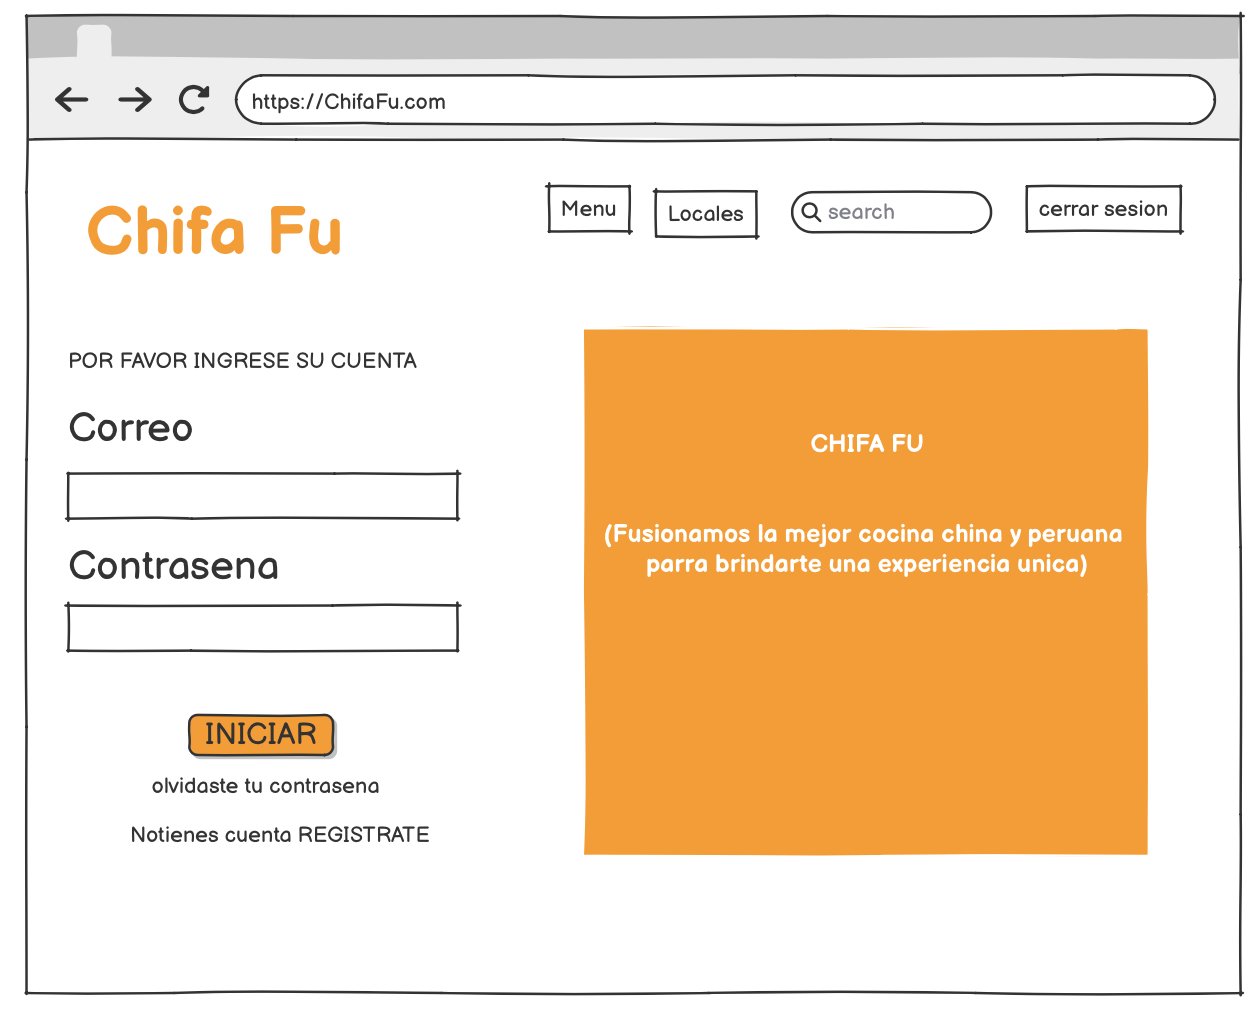
\includegraphics[width=14cm]{Solución 1/inicio.png}
        \caption{Inicio}
        \label{fig:Inicio}
    \end{figure}
    \begin{figure}[H]
        \centering
        \vspace*{1cm}
        \includegraphics[width=14cm]{Solución 1/carrito.png}
        \caption{Carrito}
        \label{fig:Carrito}
    \end{figure}
    \begin{figure}[H]
        \centering
        \vspace*{1cm}
        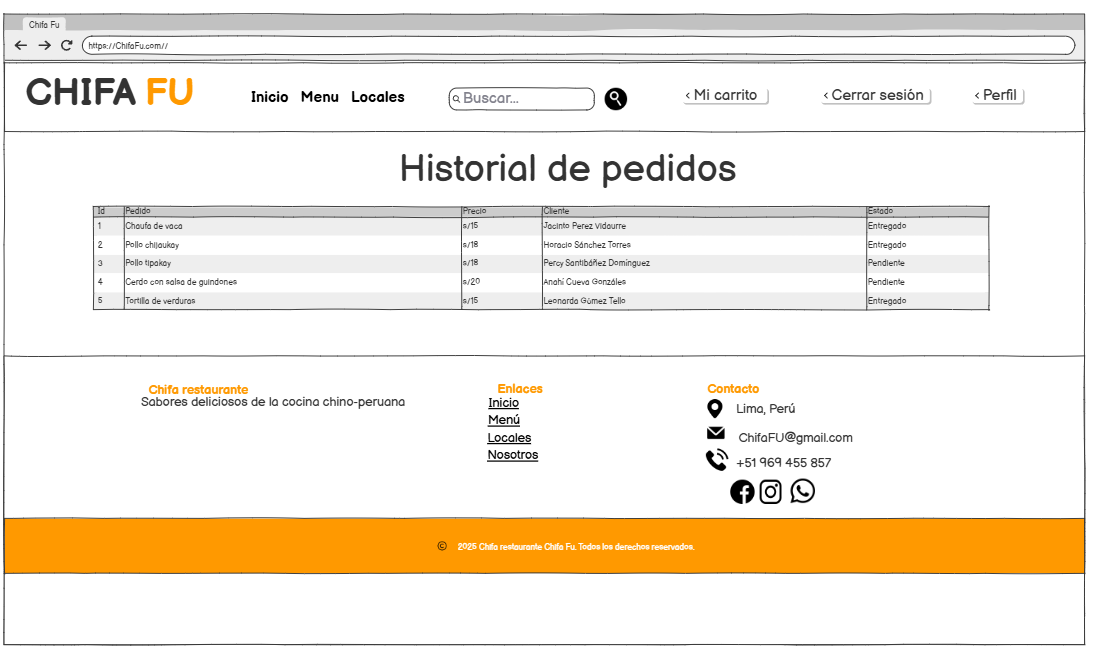
\includegraphics[width=14cm]{Solución 1/historialPedidos.png}
        \caption{Historial de pedidos}
        \label{fig:Historial-Pedidos}
    \end{figure}
    \begin{figure}[H]
        \centering
        \vspace*{1cm}
        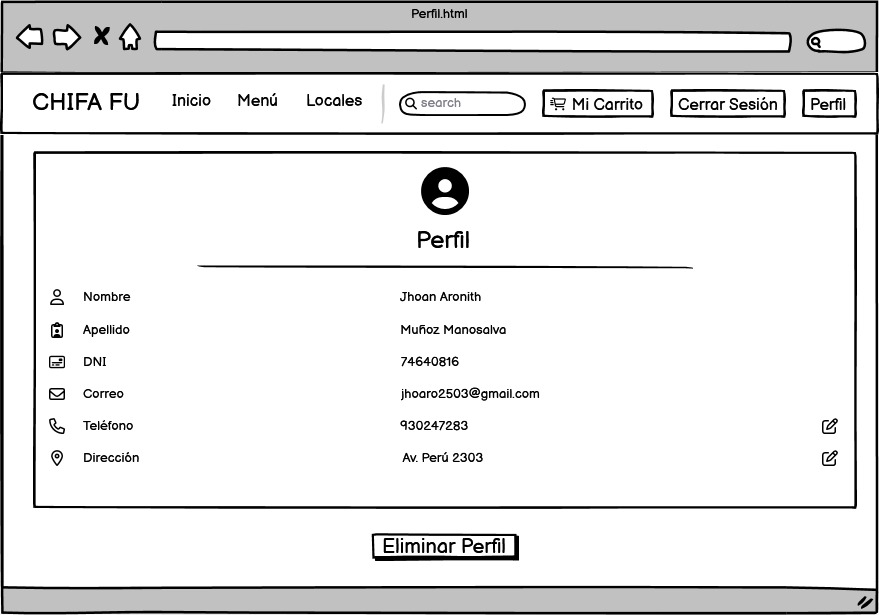
\includegraphics[width=14cm]{Solución 1/perfil.jpg}
        \caption{Perfil}
        \label{fig:Perfil}
    \end{figure}
    \begin{figure}[H]
        \centering
        \vspace*{1cm}
        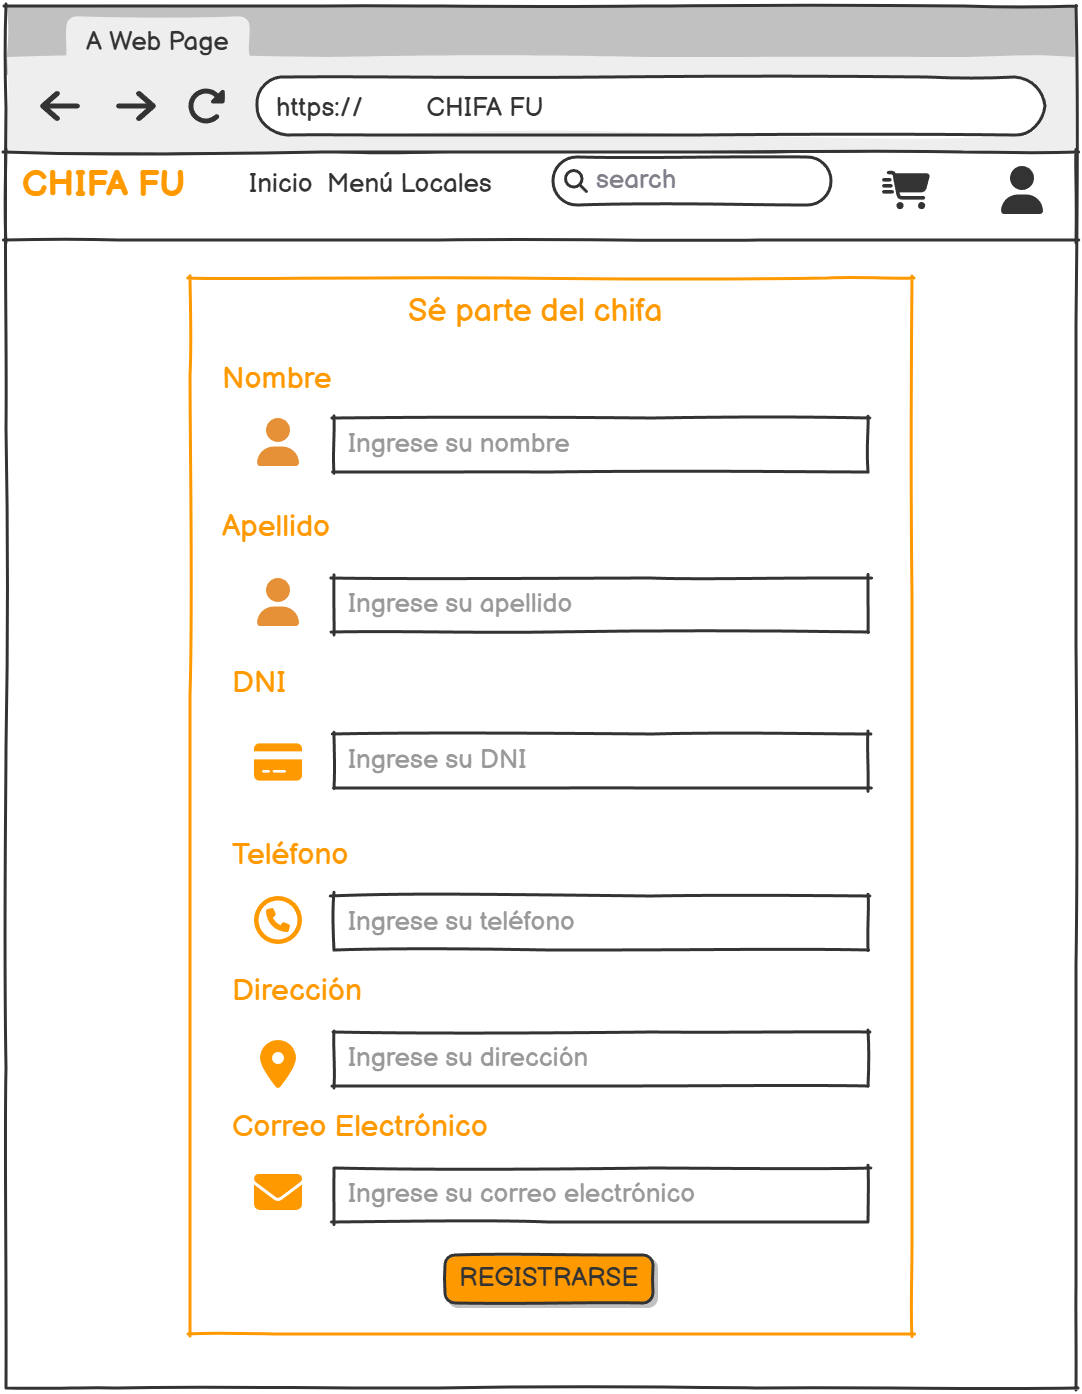
\includegraphics[width=14cm]{Solución 1/registro chifa.png}
        \caption{Registro}
        \label{fig:Registro}
    \end{figure}
    
    \subsection{Alternativa 2: Optimización de pedidos}

    \noindent Son interfaces diseñadas para hacer que el proceso de pedir sea rápido y sencillo. Incluye menú digital interactivo, carrito de compras, integración con métodos de pago, seguimiento en tiempo real e historial de pedidos.\\
    \textbf{Ventajas:}\\
    - El cliente puede personalizar su pedido fácilmente.\\
    - Pagos más ágiles gracias a la integración con billeteras digitales y tarjetas.\\
    - Mayor fidelización al permitir repetir pedidos anteriores con un clic.\\
    - Transparencia y confianza al mostrar el seguimiento del pedido en tiempo real.\\
    \textbf{Desventajas:}\\
    - Depende de una buena conexión a internet.\\
    - Algunos clientes tradicionales pueden resistirse a usar un sistema digital.\\
    - Costos de integración con pasarelas de pago externas.\\

    \begin{figure}[H]
        \centering
        \vspace*{1cm}
        \includegraphics[width=14cm]{Solución 2/carrito.png}
        \caption{Carrito}
        \label{fig:Carrito}
    \end{figure}
    \begin{figure}[H]
        \centering
        \vspace*{1cm}
        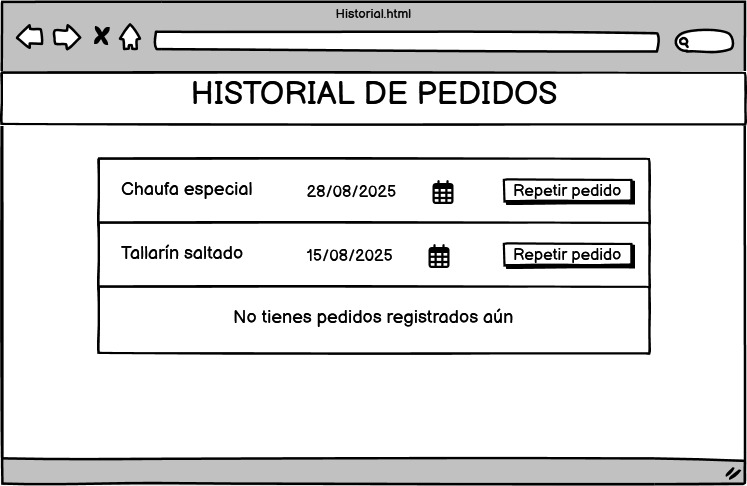
\includegraphics[width=14cm]{Solución 2/historial.jpg}
        \caption{Historial}
        \label{fig:Historial}
    \end{figure}
    \begin{figure}[H]
        \centering
        \vspace*{1cm}
        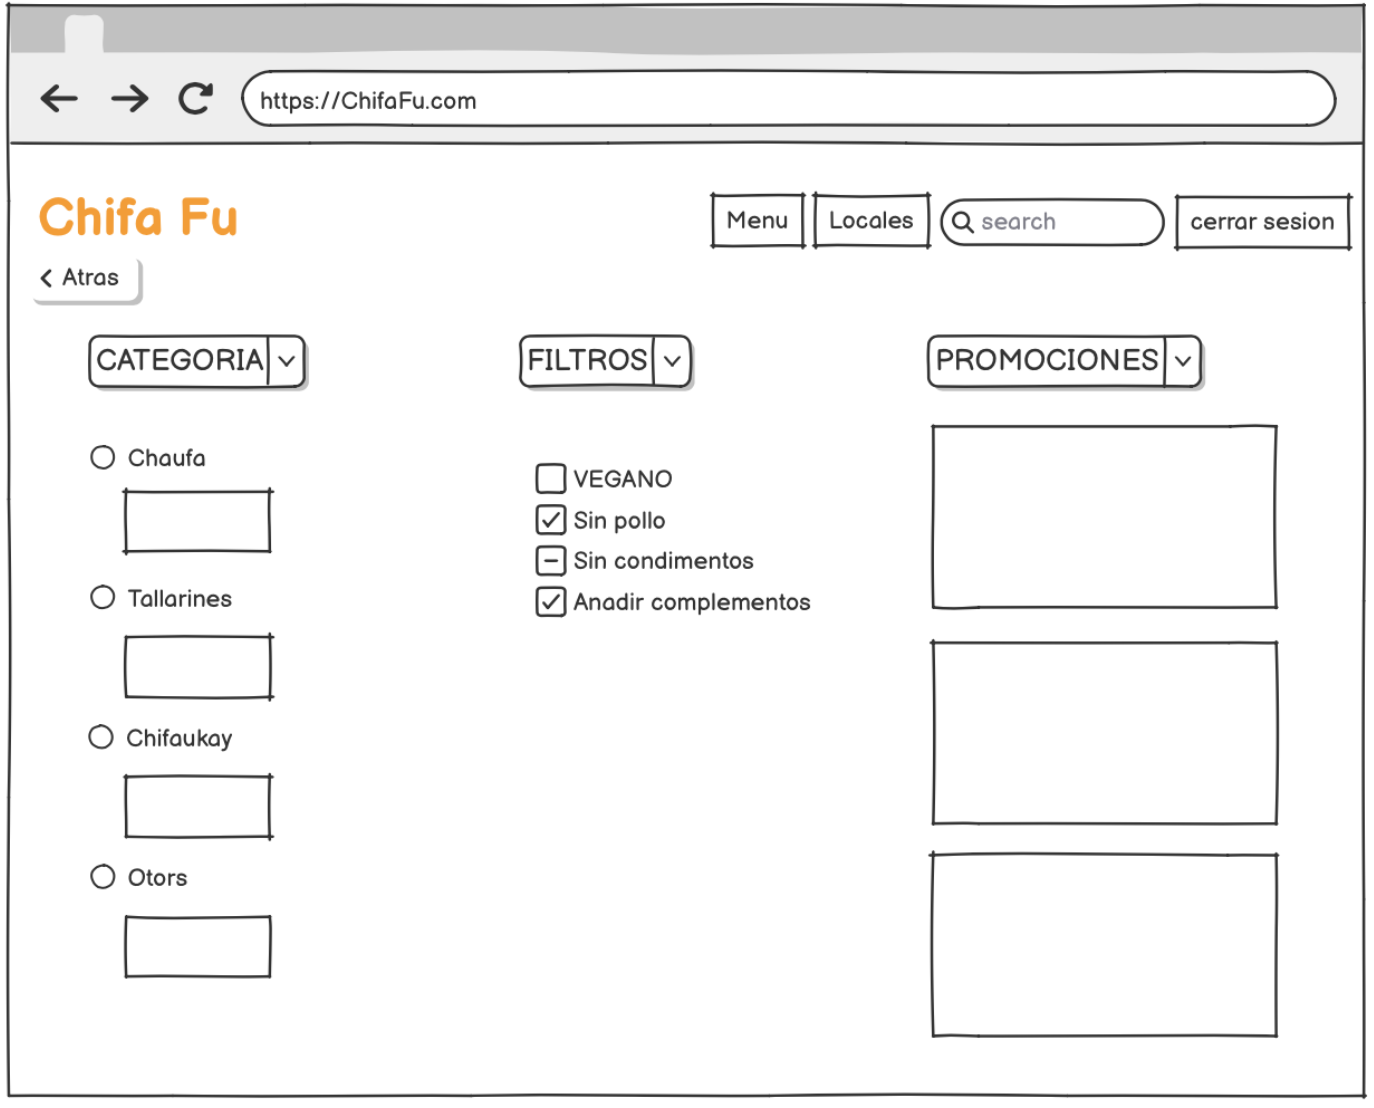
\includegraphics[width=14cm]{Solución 2/menudigital.png}
        \caption{Menu Digital}
        \label{fig:Menu-Digital}
    \end{figure}
    \begin{figure}[H]
        \centering
        \vspace*{1cm}
        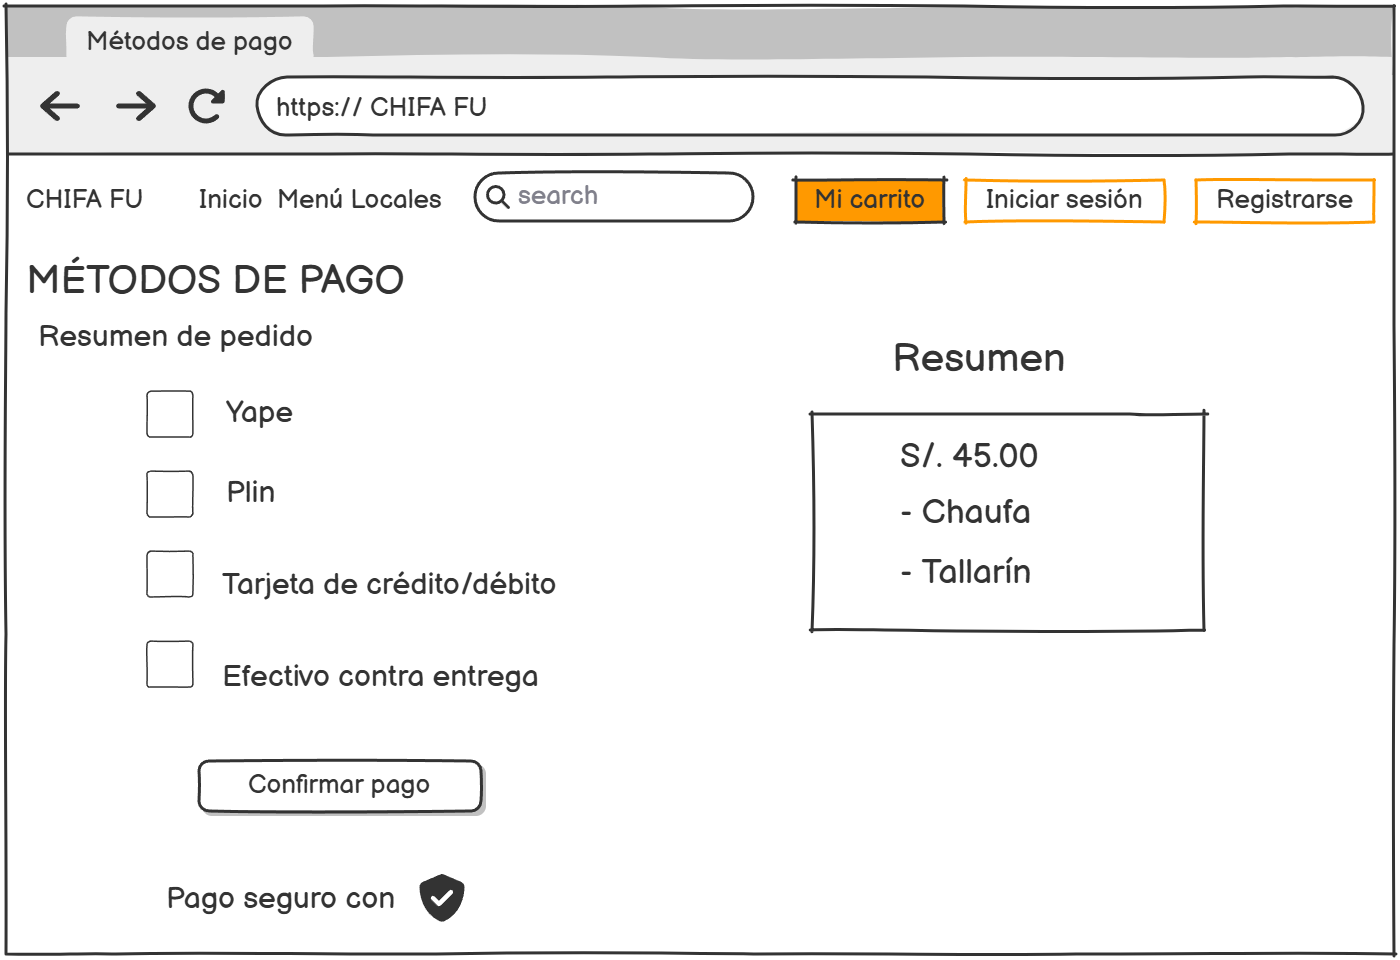
\includegraphics[width=14cm]{Solución 2/metodos de pago.png}
        \caption{metodos de pago}
        \label{fig:Metodos-de-pago}
    \end{figure}
    \begin{figure}[H]
        \centering
        \vspace*{1cm}
        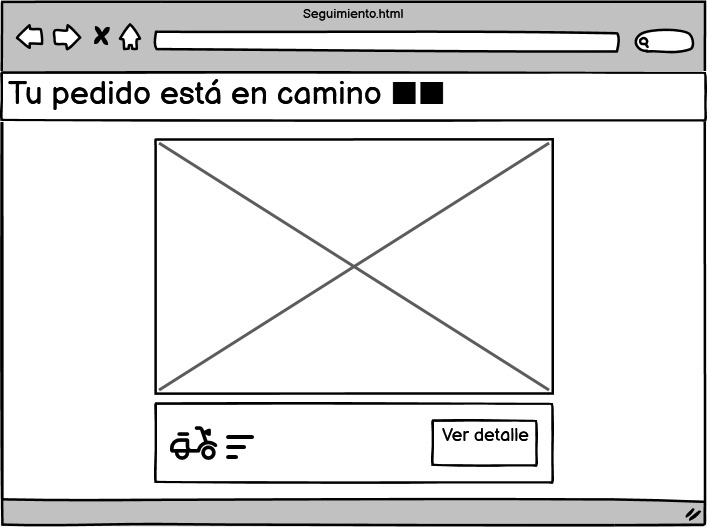
\includegraphics[width=14cm]{Solución 2/seguimiento.jpg}
        \caption{Seguimiento}
        \label{fig:Seguimiento}
    \end{figure}
    
    \subsection{Alternativa 3: Administrador}

    \noindent Se propone el desarrollo de un módulo administrador dentro del sistema web, orientado exclusivamente al personal autorizado. Este módulo centralizará la gestión y el control del restaurante, permitiendo administrar usuarios, productos del menú, promociones, inventario, historial de ventas y estadísticas en tiempo real. Además, permitirá configurar parámetros del sistema, garantizando un entorno de trabajo digital ordenado y eficiente.\\
    \textbf{Ventajas:}\\
    - Control centralizado: Permite al restaurante gestionar todos los aspectos del negocio desde una sola plataforma.\\
    - Toma de decisiones informada: El acceso a reportes automáticos de ventas, consumo e inventario brinda datos clave para definir estrategias comerciales.\\
    - Gestión de roles y seguridad: El administrador podrá asignar permisos diferenciados, reforzando la confiabilidad del sistema.\\
    \textbf{Desventajas:}\\
    - Complejidad inicial: El personal administrativo requiere capacitación para manejar todas las funcionalidades correctamente.\\
    - Dependencia tecnológica: Fallos en el sistema pueden afectar la operatividad del restaurante en su totalidad.\\
    - Costos de implementación y soporte: Involucra inversión en servidores, mantenimiento y actualizaciones periódicas.\\

    \begin{figure}[H]
        \centering
        \vspace*{1cm}
        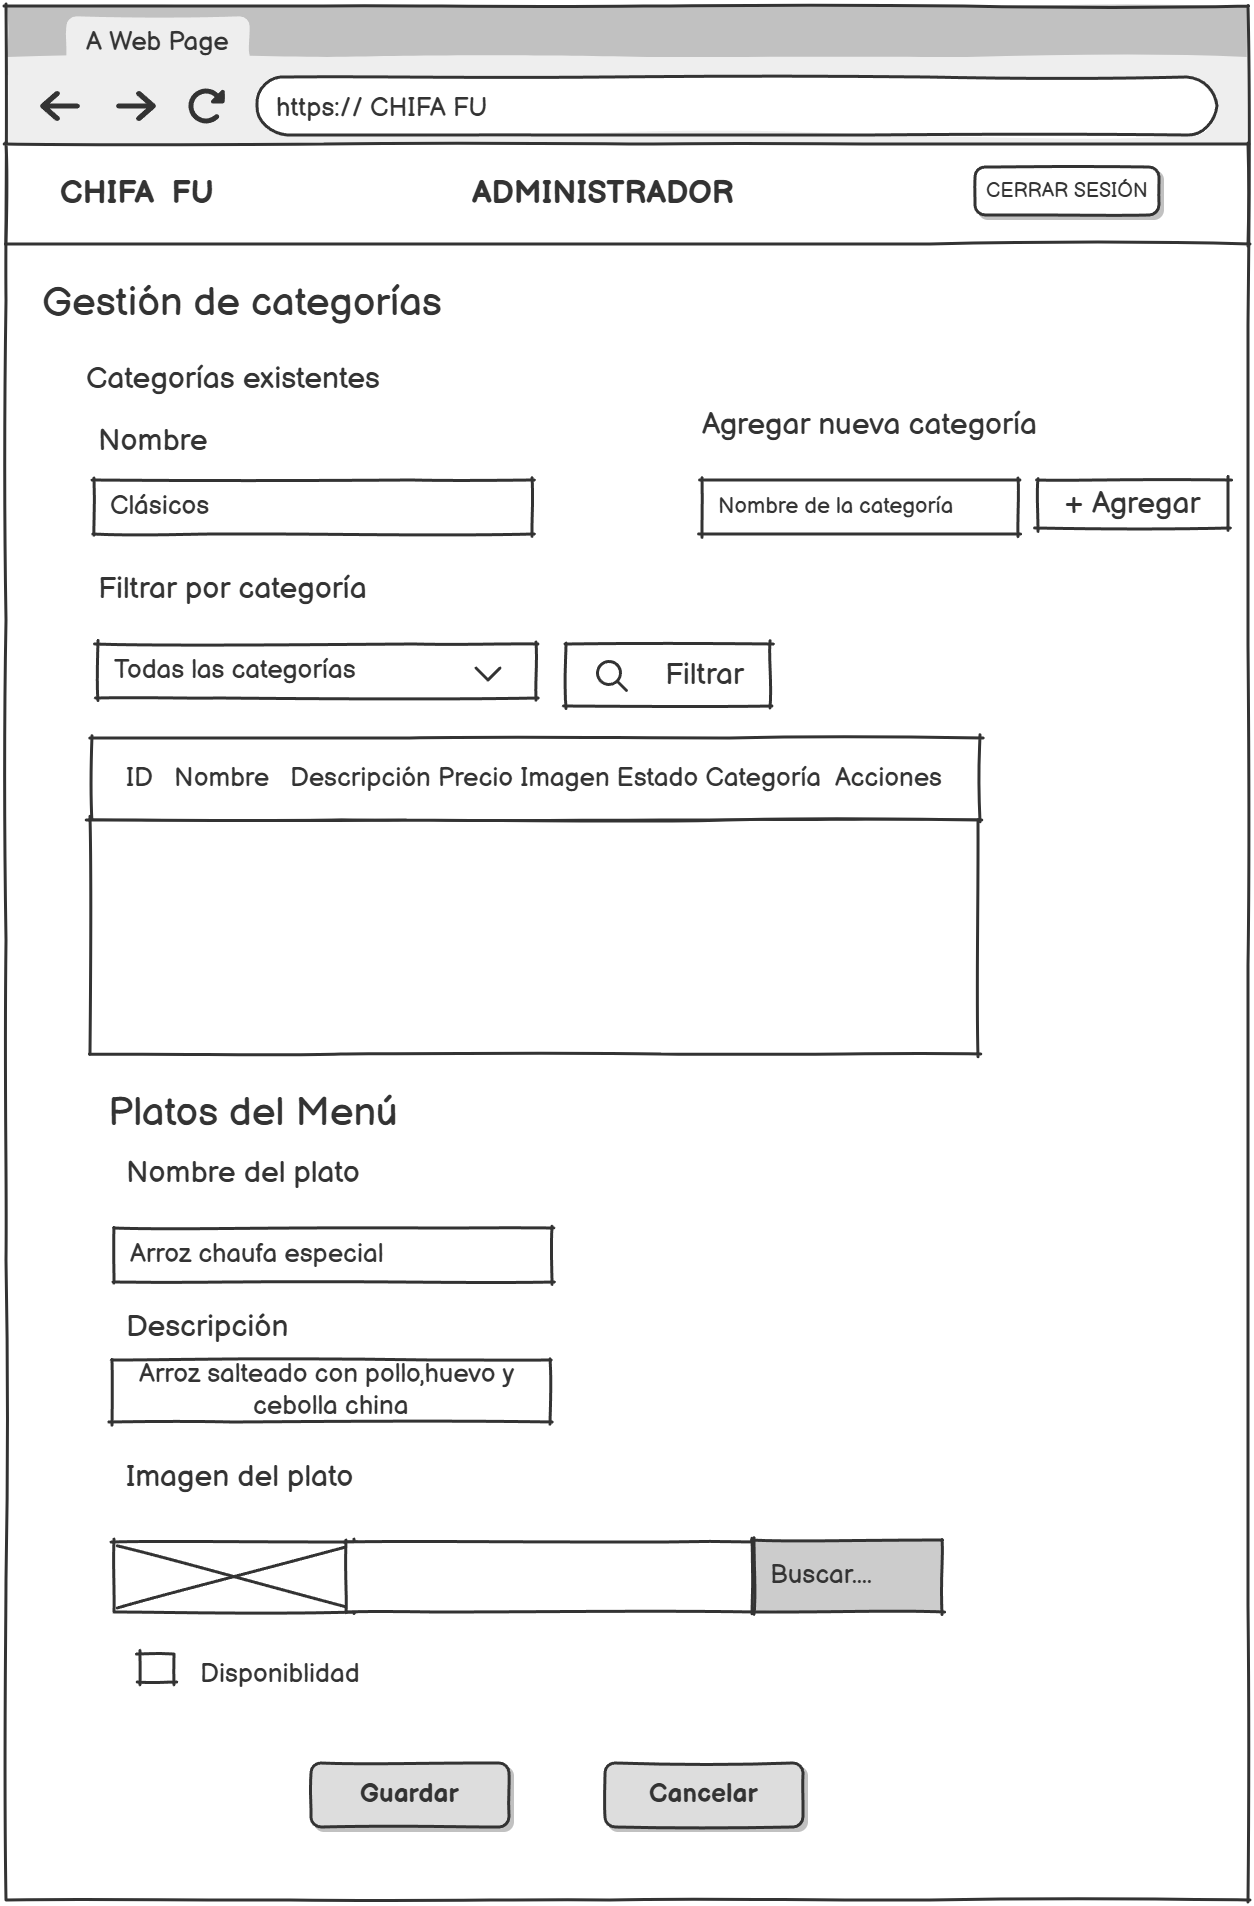
\includegraphics[width=14cm]{Solución 3/formulario menus.png}
        \caption{Formulario Menu}
        \label{fig:formulario-menu}
    \end{figure}
    \begin{figure}[H]
        \centering
        \vspace*{1cm}
        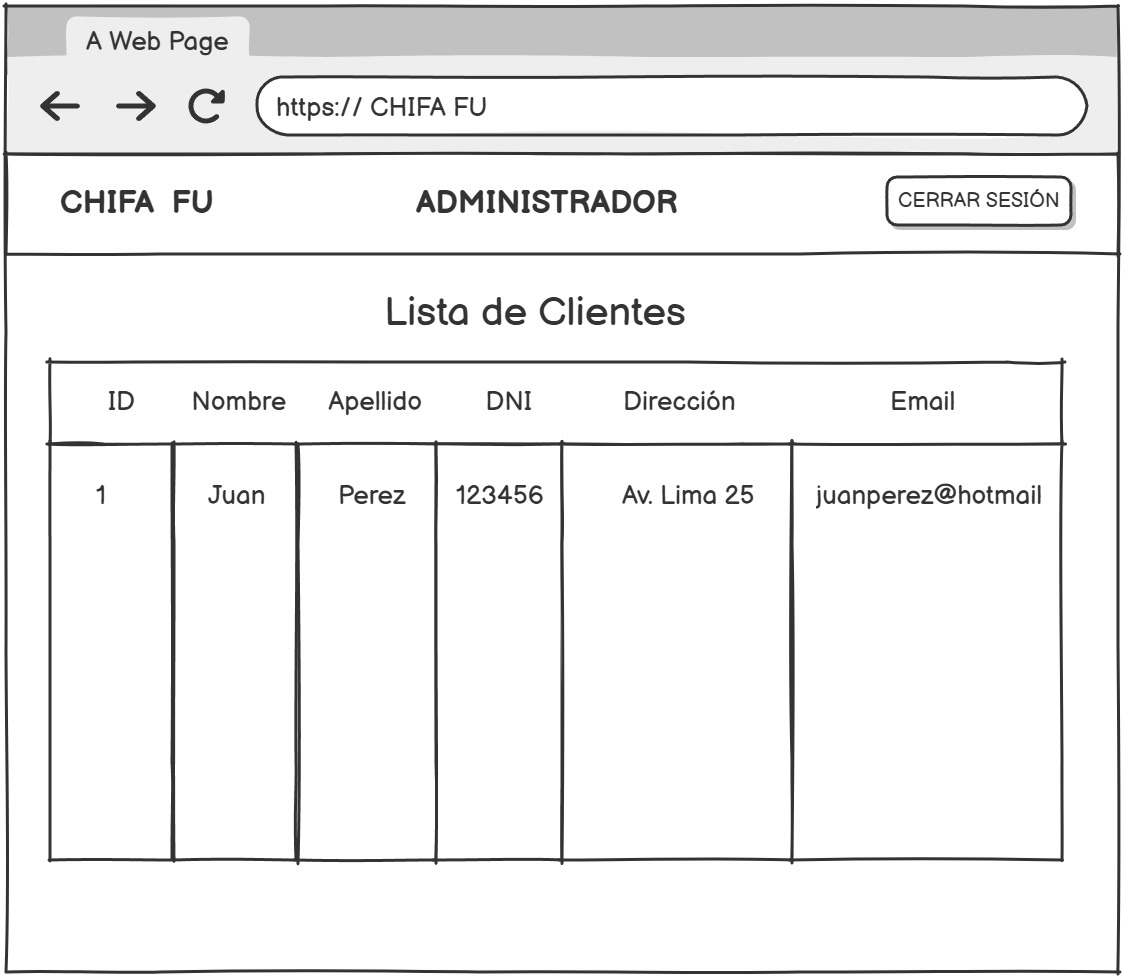
\includegraphics[width=14cm]{Solución 3/listaclientes_admi.jpeg}
        \caption{Lista de clientes}
        \label{fig:lista-clientes}
    \end{figure}
    \begin{figure}[H]
        \centering
        \vspace*{1cm}
        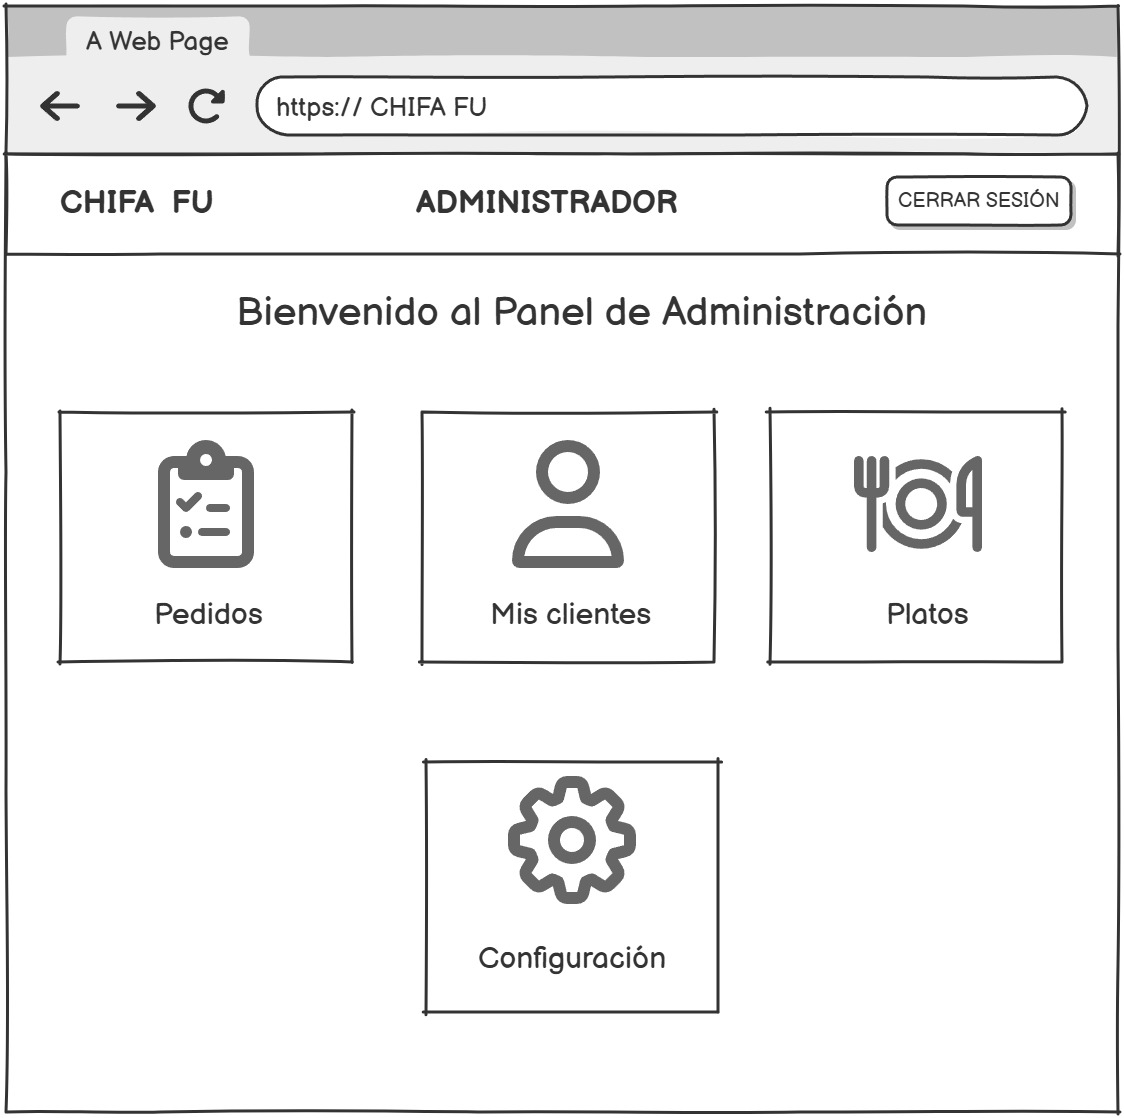
\includegraphics[width=14cm]{Solución 3/panel_admi.jpeg}
        \caption{Panel administrador}
        \label{fig:panel-admin}
    \end{figure}
    \begin{figure}[H]
        \centering
        \vspace*{1cm}
        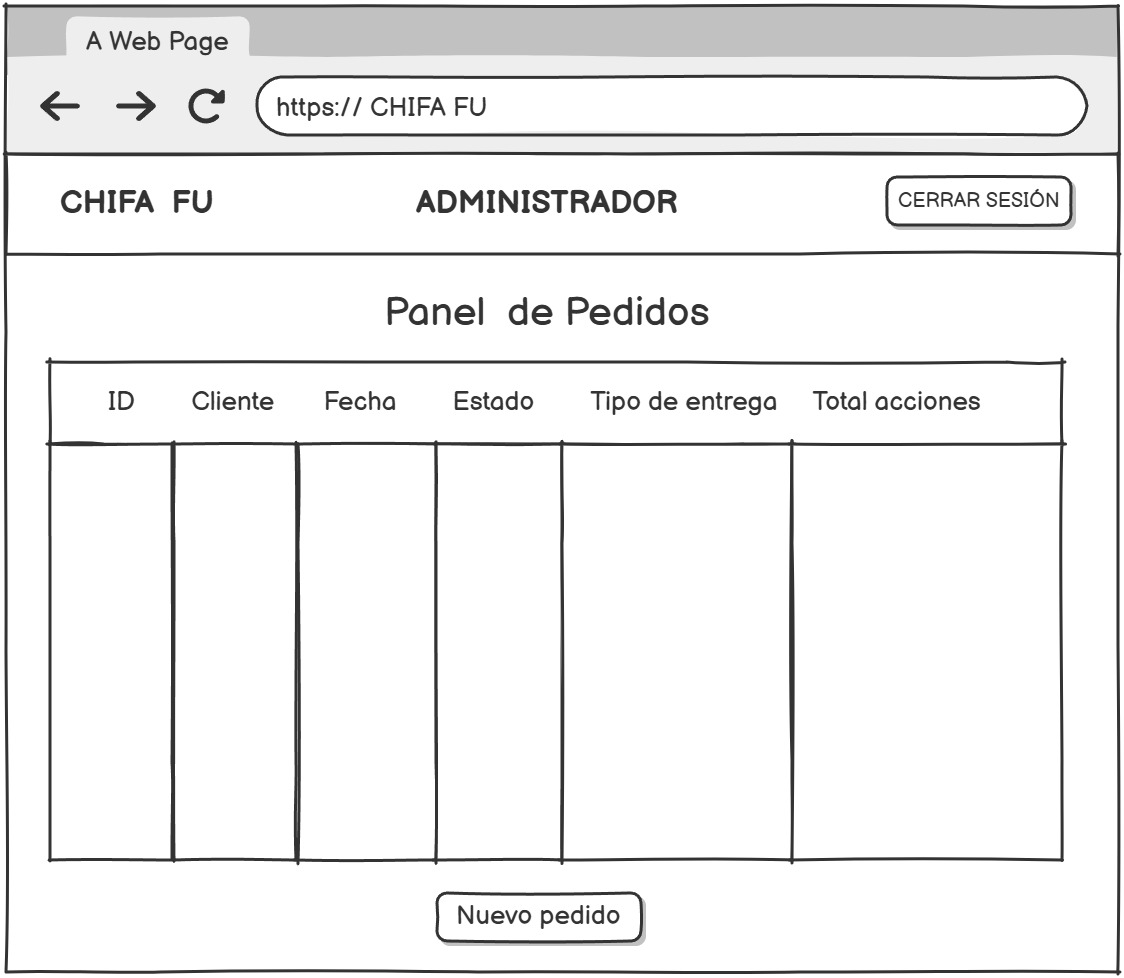
\includegraphics[width=14cm]{Solución 3/panelpedidos_admi.jpeg}
        \caption{Panel de pedidos}
        \label{fig:panel-pedidos}
    \end{figure}
    \begin{figure}[H]
        \centering
        \vspace*{1cm}
        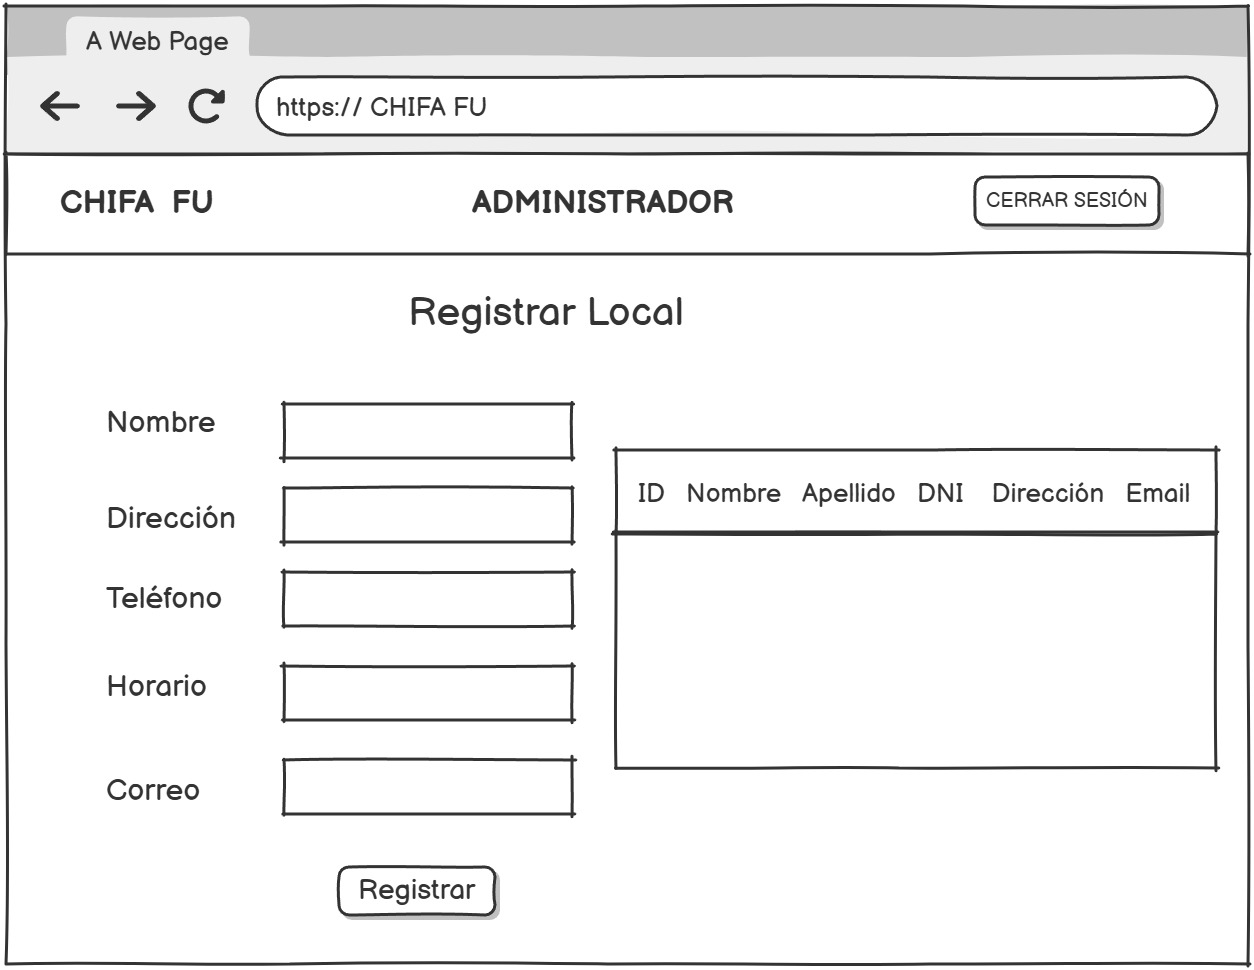
\includegraphics[width=14cm]{Solución 3/registrolocal_admi.jpeg}
        \caption{Registro local}
        \label{fig:registro-local}
    \end{figure}

     \section{Casos de uso}
    \noindent 
    Actores: Cliente, Administrador.\\
    Estados estándar de pedido: pendiente → en preparación → listo → entregado.\\
    
    UC-01: Registrarse\\
    - Actor: Cliente\\
    - Objetivo: Crear cuenta para pedidos e historial.\\
    - Pre: No autenticado.\\
    - Flujo básico: (1) Abre “Registrarse” → (2) Ingresa datos → (3) Sistema valida → (4) Crea cuenta → (5) Confirma.\\
    - Post: Cuenta activa; sesión iniciada.\\
    - Excepciones: E1 correo ya registrado; E2 contraseña débil → mostrar mensaje.\\
    
    UC-02: Iniciar sesión\\
    - Actor: Cliente / Administrador\\
    - Objetivo: Autenticarse en el sistema.\\
    - Flujo: Ingresa credenciales → Validación → Acceso según rol.\\
    - Post: Sesión activa con permisos del rol.\\
    - Excepciones: E1 credenciales inválidas; E2 cuenta bloqueada.\\
    
    UC-03: Visualizar menú\\
    - Actor: Cliente\\
    - Objetivo: Ver platos disponibles con info clave.\\
    - Flujo: Entra a “Menú” → El sistema lista categorías/platos → (opcional) buscar/filtrar.\\
    - Post: Menú mostrado con disponibilidad actual.\\
    
    UC-04: Gestionar carrito\\
    - Actor: Cliente\\
    - Objetivo: Armar y ajustar el pedido.\\
    - Flujo: Desde menú agrega/edita/elimina ítems → Ve total y resumen.\\
    - Post: Carrito persistido en sesión.\\
    - Excepciones: E1 plato sin stock → sugerir alternativa.\\

    UC-05: Realizar pedido en línea\\
    - Actor: Cliente\\
    - Objetivo: Confirmar y registrar pedido.\\
    - Pre: UC-04 completado.\\
    - Flujo: (1) Revisa carrito → (2) Ingresa datos de entrega/sede y notas → (3) Confirma → (4) Sistema registra y devuelve N° de orden.\\
    - Post: Pedido en estado pendiente.\\
    - Excepciones: E1 validación de datos; E2 fallo de registro → reintento y mensaje.\\
    
    UC-06: Seguir estado del pedido\\
    - Actor: Cliente\\
    - Objetivo: Ver progreso en tiempo (casi) real.\\
    - Pre: Pedido existente.\\
    - Flujo: Abre “Mis pedidos” → Selecciona orden → Visualiza estado y tiempos estimados.\\
    - Post: Estado visible actualizado.\\

    UC-07: Ver historial y repetir pedido\\
    - Actor: Cliente\\
    - Objetivo: Reordenar rápido.\\
    - Flujo: “Historial” → Elige pedido → “Repetir” → Sistema crea nuevo carrito con mismos ítems (usuario puede editar).\\
    - Post: Carrito precargado listo para UC-05.\\
    
    UC-08: Editar perfil\\
    - Actor: Cliente\\
    - Objetivo: Actualizar datos de cuenta.\\
    - Flujo: Abre “Perfil” → Edita → Guarda → Confirmación.\\
    - Post: Datos actualizados.\\

    UC-09: Gestionar pedidos (Admin)\\
    - Actor: Administrador\\
    - Objetivo: Controlar el flujo operativo de pedidos.\\
    - Pre: Autenticado con rol Admin.\\
    - Flujo: “Panel de pedidos” → Lista pedidos → Cambia estado (pendiente/en preparación/listo/entregado) → Sistema notifica al cliente/actualiza vista.\\
    - Post: Estado actualizado; registro en auditoría.\\
    - Excepciones: E1 intento de cambio inválido; E2 pedido inexistente.\\

    UC-10: Administrar menú (CRUD)\\
    - Actor: Administrador\\
    - Objetivo: Mantener platos y precios.\\
    - Flujo: “Menú (admin)” → Crear/editar/desactivar plato → Guardar.\\
    - Post: Menú público actualizado.\\
    - Excepciones: E1 datos incompletos; E2 imagen inválida.\\
    - UC-11: Administrar promociones/contenido\\
    - Actor: Administrador\\
    - Objetivo: Gestionar promos visibles en área pública.\\
    - Flujo: Crear/editar promo (vigencia, precio/combo) → Publicar/retirar.\\
    - Post: Sitio muestra promos vigentes.\\

    UC-12: Gestionar inventario\\
    - Actor: Administrador\\
    - Objetivo: Control de stock.\\
    - Post: Stock actualizado; impacto en disponibilidad de platos.\\

    UC-13: Gestionar usuarios y roles\\
    - Actor: Administrador\\
    - Objetivo: Alta/baja/modificación de usuarios internos y permisos.\\
    - Flujo: “Usuarios” → Crear usuario (rol: mesero/cocina/reparto/gerencia) o editar permisos → Guardar.\\
    - Post: Accesos aplicados según RBAC.\\

\section{Diagrama Gantt}
    \noindent Aplicaremos el Diagrama de Gantt para planificar la ejecución y las etapas de nuestro proyecto.
    \begin{figure}[H]
        \centering
        \vspace*{1cm}
        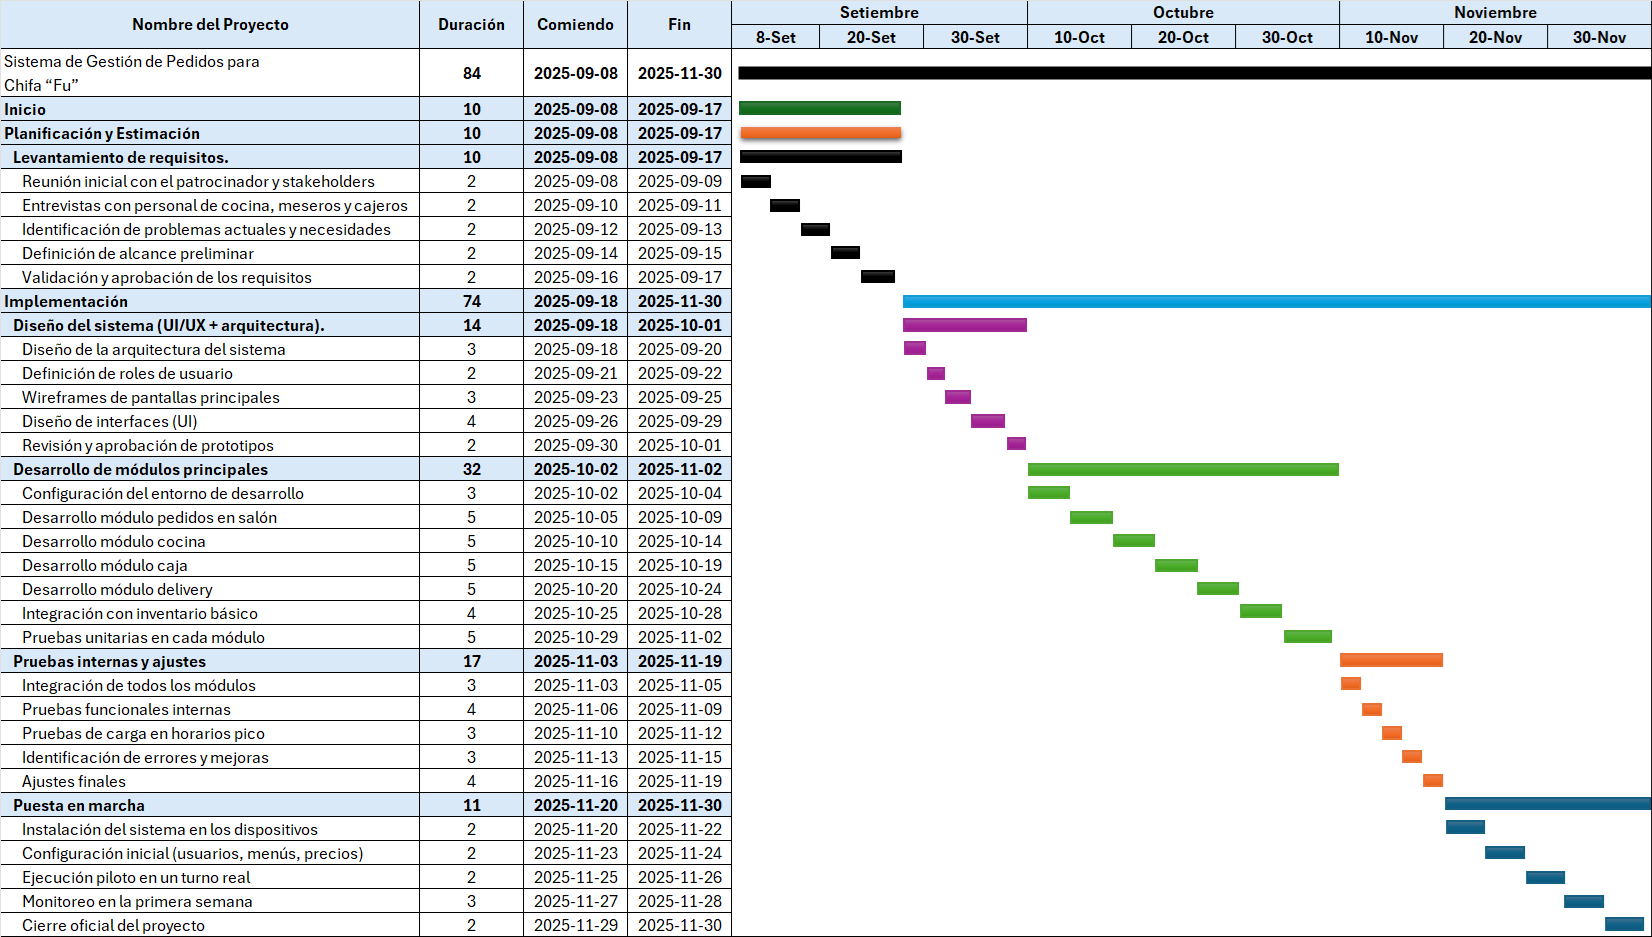
\includegraphics[width=14cm]{Gantt, WBS, Project Charter, BPM/gantt.png}
        \caption{Diagrama Gantt}
        \label{fig:Diagrama-gantt}
    \end{figure}

\section{Project Charter}

\begin{figure}[H]
    \centering
    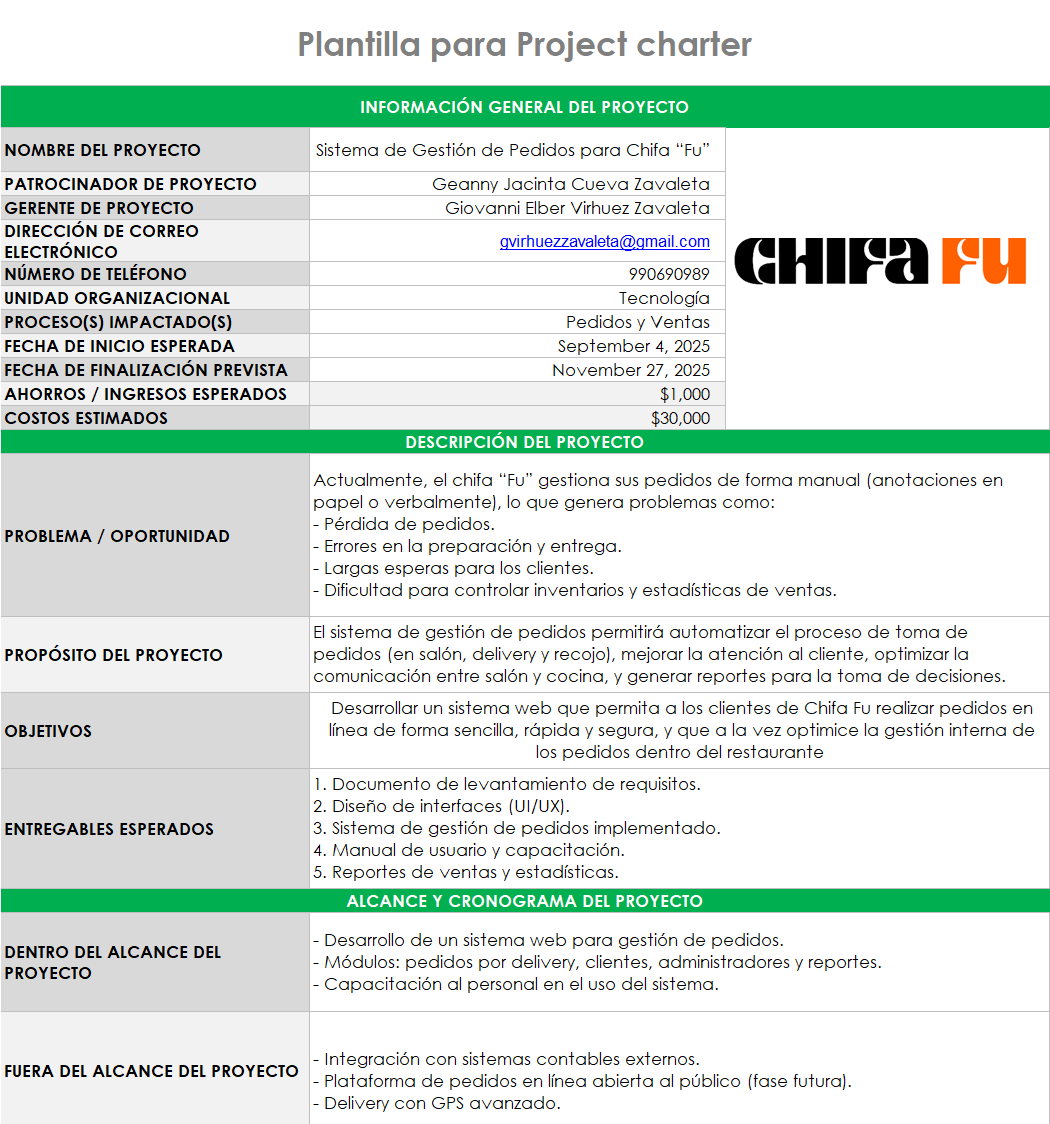
\includegraphics[width=\textwidth]{Gantt, WBS, Project Charter, BPM/projectCharter1.png}
    \label{fig:Project-Charter}
\end{figure}

\begin{figure}[H]
    \centering
    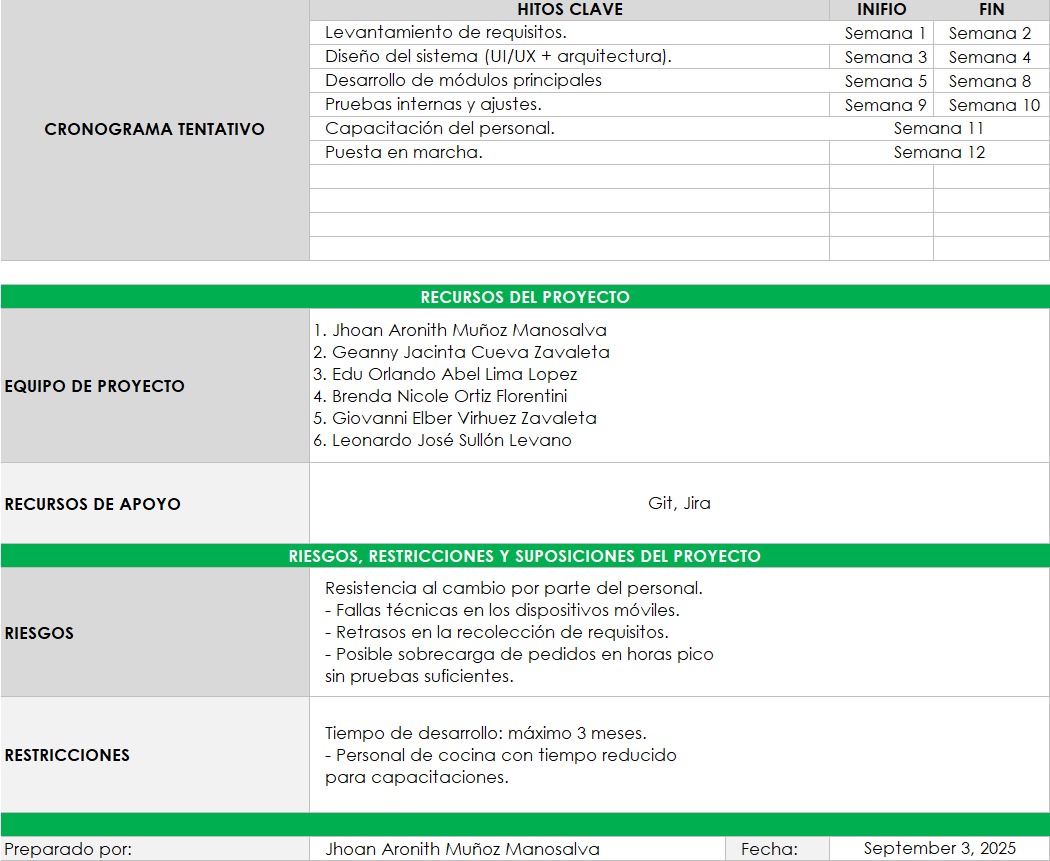
\includegraphics[width=\textwidth]{Gantt, WBS, Project Charter, BPM/projectCharter2.png}
    \caption{Project Charter}
    \label{fig:Project-Charter}
\end{figure}


\section{Estructura de desglose del trabajo (WBS)}

    \begin{figure}[H]
        \centering
        \vspace*{1cm}
        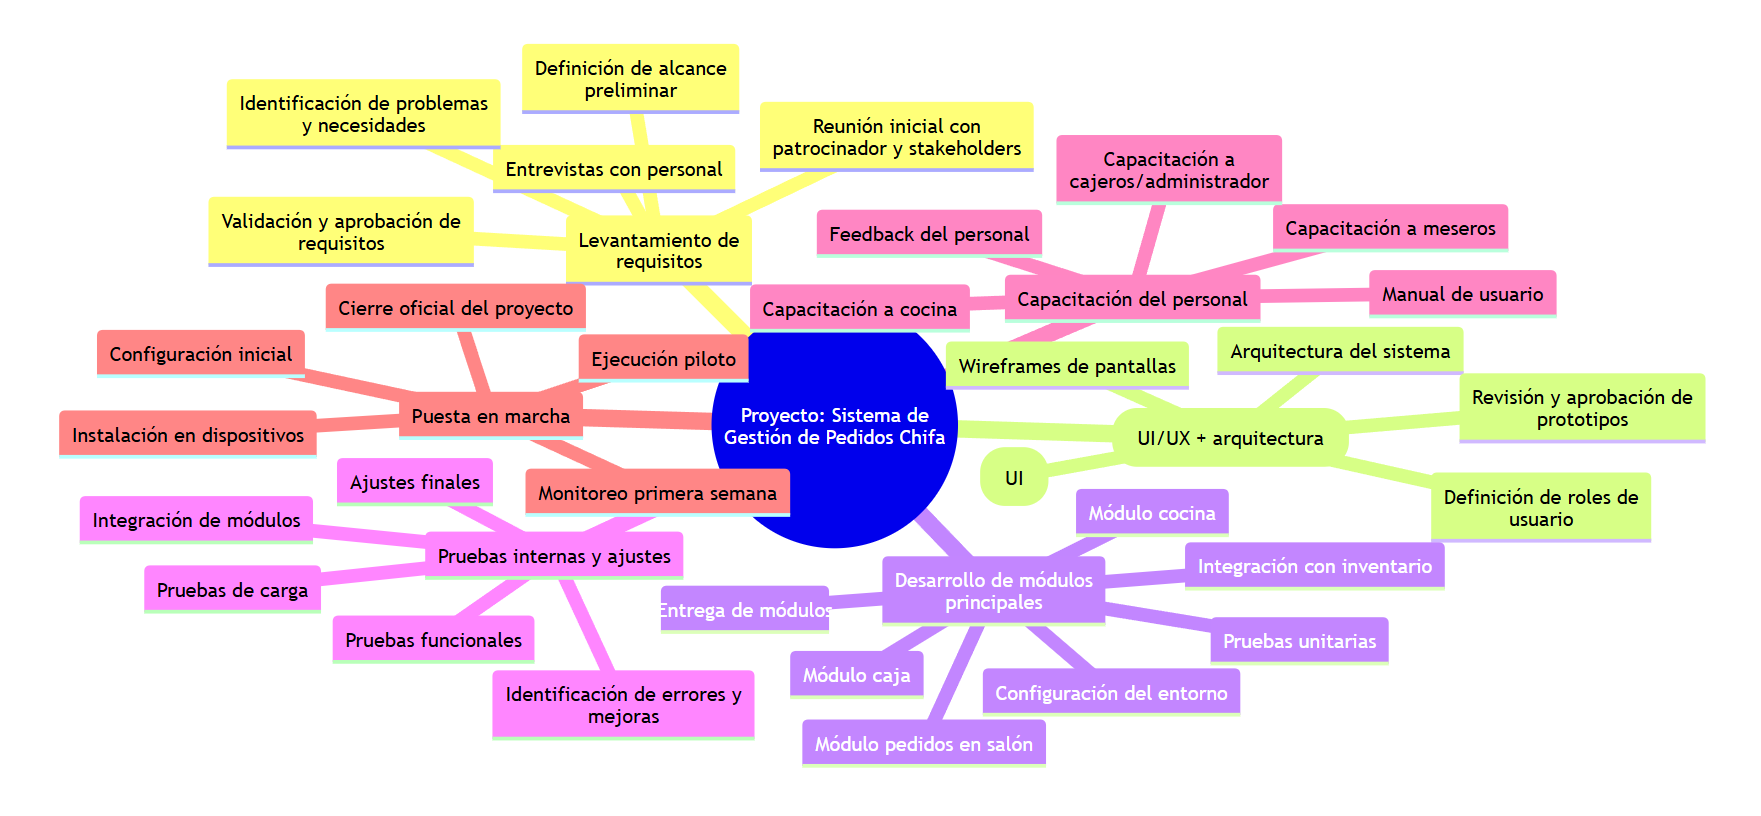
\includegraphics[width=14cm]{Gantt, WBS, Project Charter, BPM/WBS.png}
        \caption{WBS}
        \label{fig:WBS}
    \end{figure}

\section{Alternativa elegida: Alternativa 1}

    \begin{figure}[H]
        \centering
        \vspace*{1cm}
        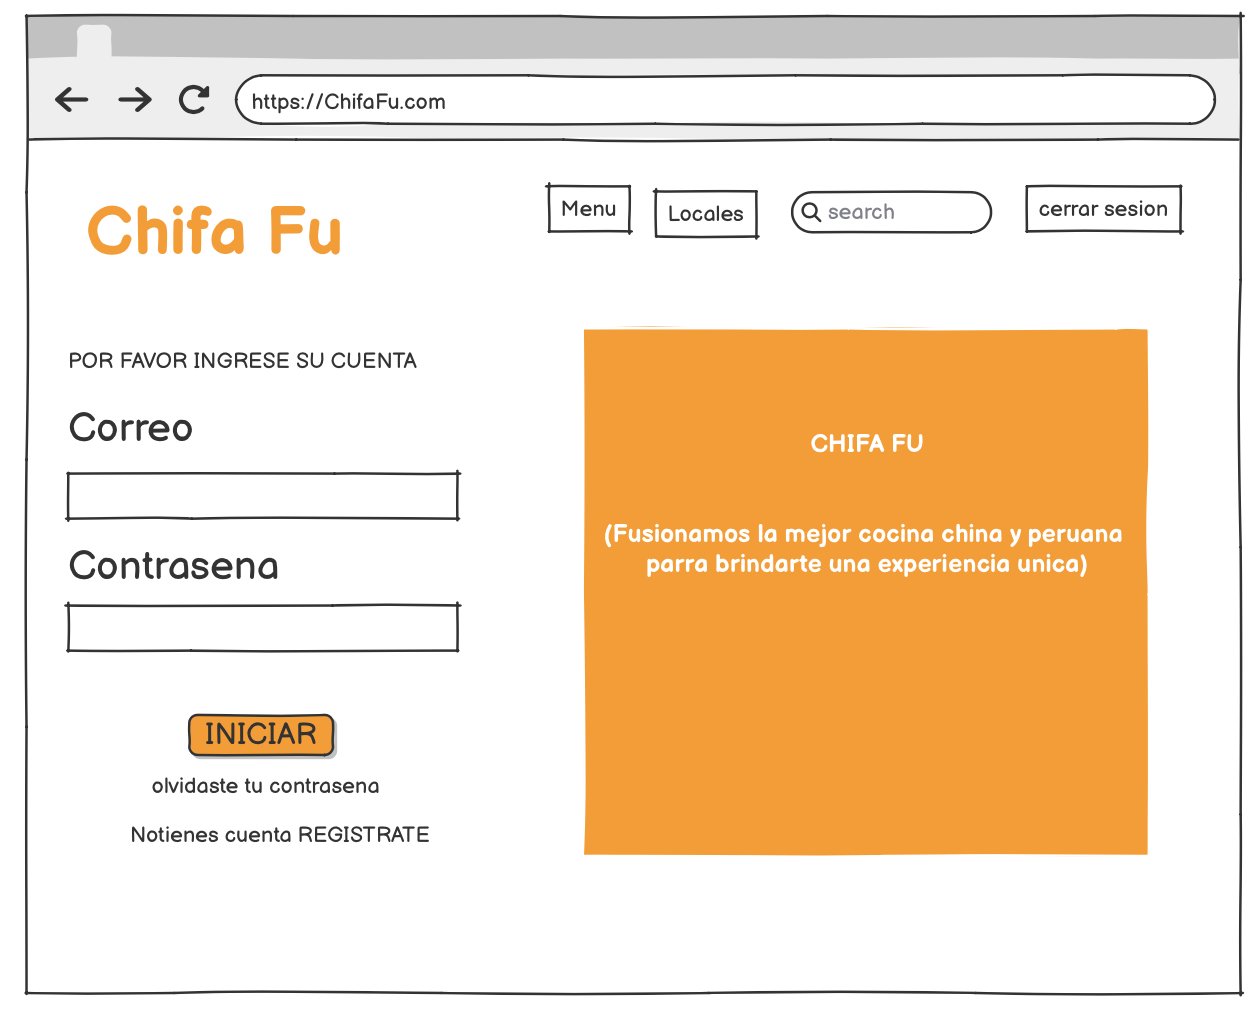
\includegraphics[width=14cm]{Solución 1/inicio.png}
        \caption{Inicio}
        \label{fig:Inicio}
    \end{figure}
    \begin{figure}[H]
        \centering
        \vspace*{1cm}
        \includegraphics[width=14cm]{Solución 1/carrito.png}
        \caption{Carrito}
        \label{fig:Carrito}
    \end{figure}
    \begin{figure}[H]
        \centering
        \vspace*{1cm}
        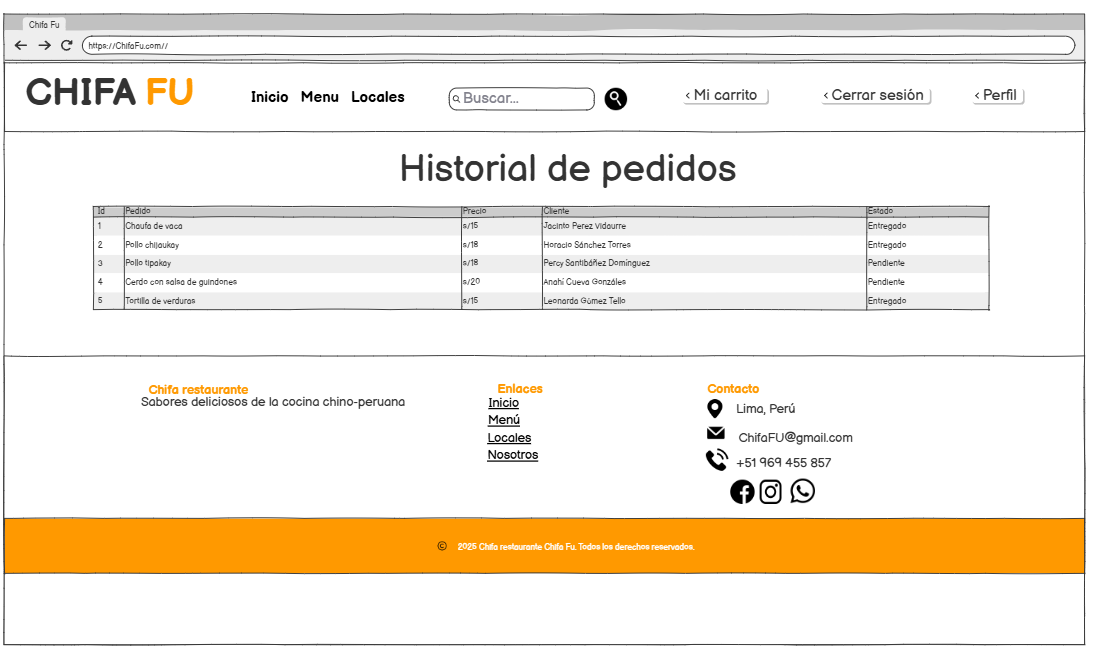
\includegraphics[width=14cm]{Solución 1/historialPedidos.png}
        \caption{Historial de pedidos}
        \label{fig:Historial-Pedidos}
    \end{figure}
    \begin{figure}[H]
        \centering
        \vspace*{1cm}
        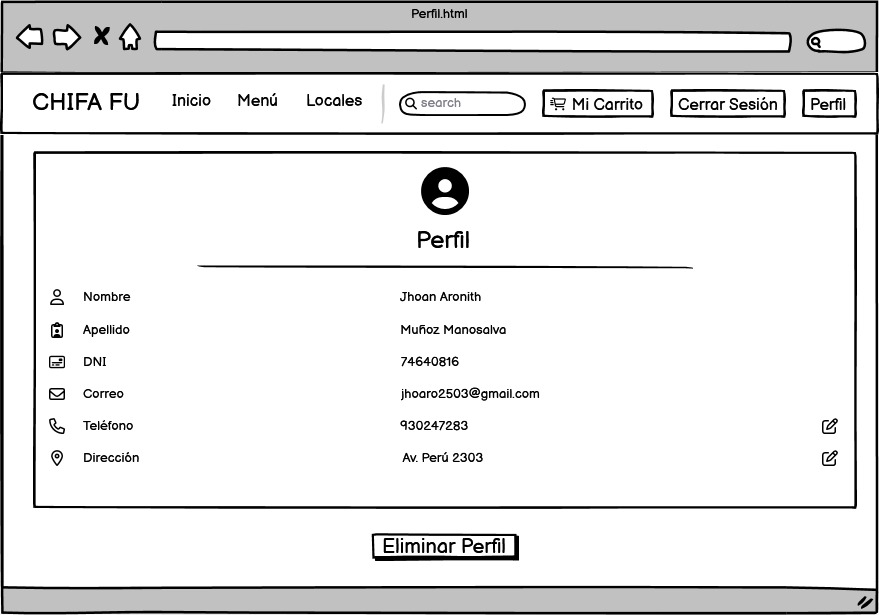
\includegraphics[width=14cm]{Solución 1/perfil.jpg}
        \caption{Perfil}
        \label{fig:Perfil}
    \end{figure}
    \begin{figure}[H]
        \centering
        \vspace*{1cm}
        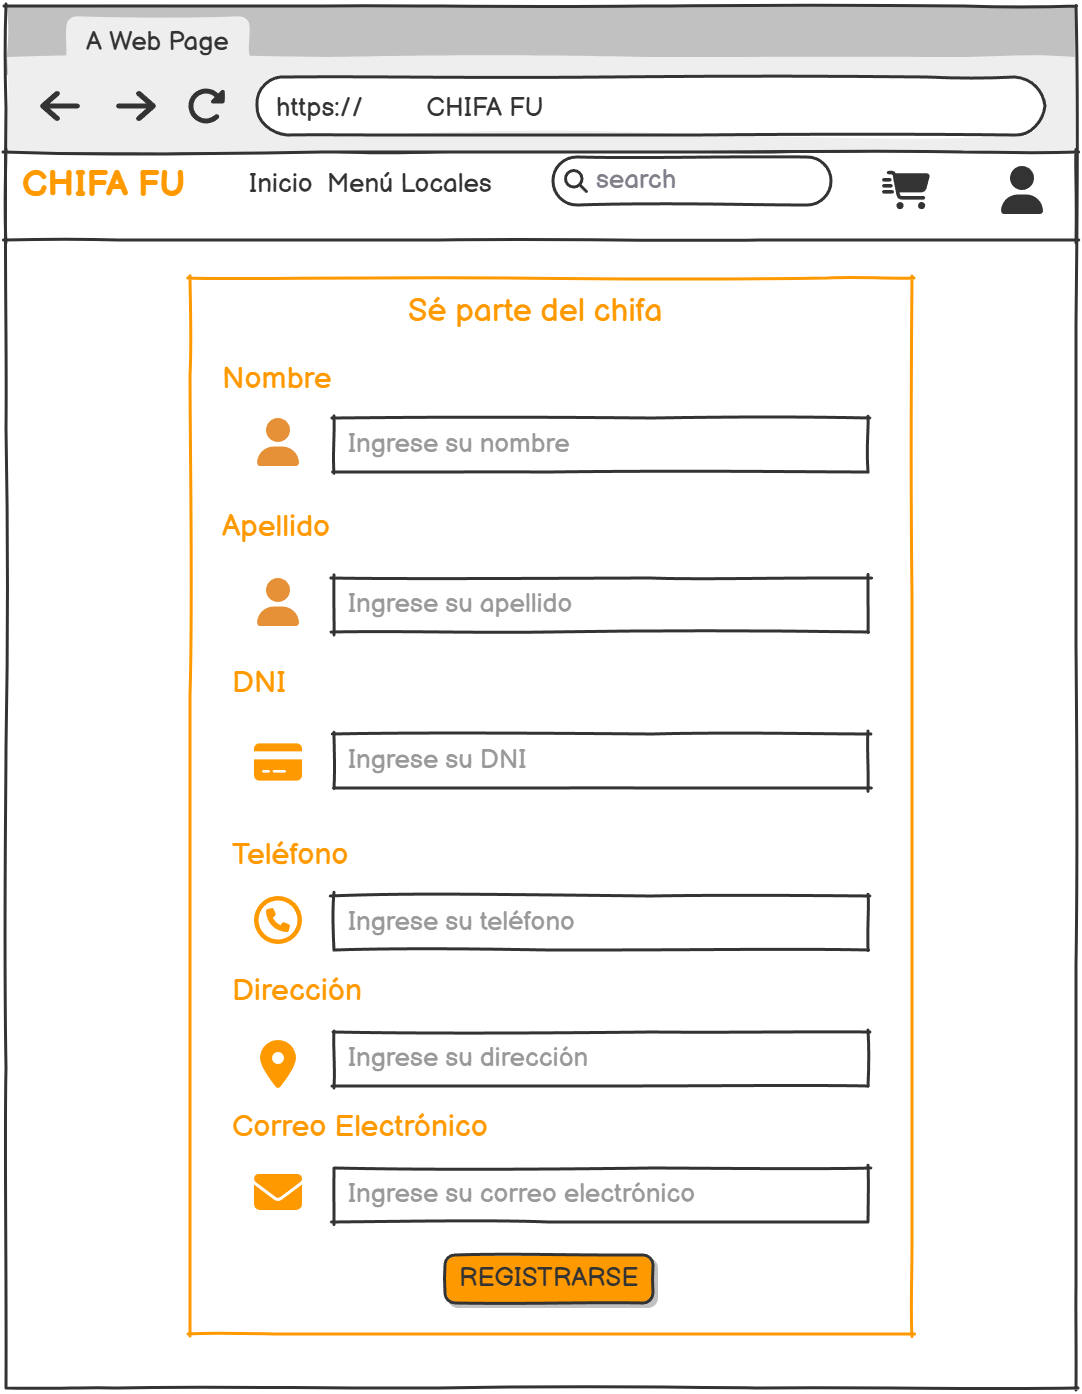
\includegraphics[width=14cm]{Solución 1/registro chifa.png}
        \caption{Registro}
        \label{fig:Registro}
    \end{figure}

    \section{Modelado BPM}
    \begin{itemize}
        \begin{figure}[H]
            \centering
            \vspace*{1cm}
            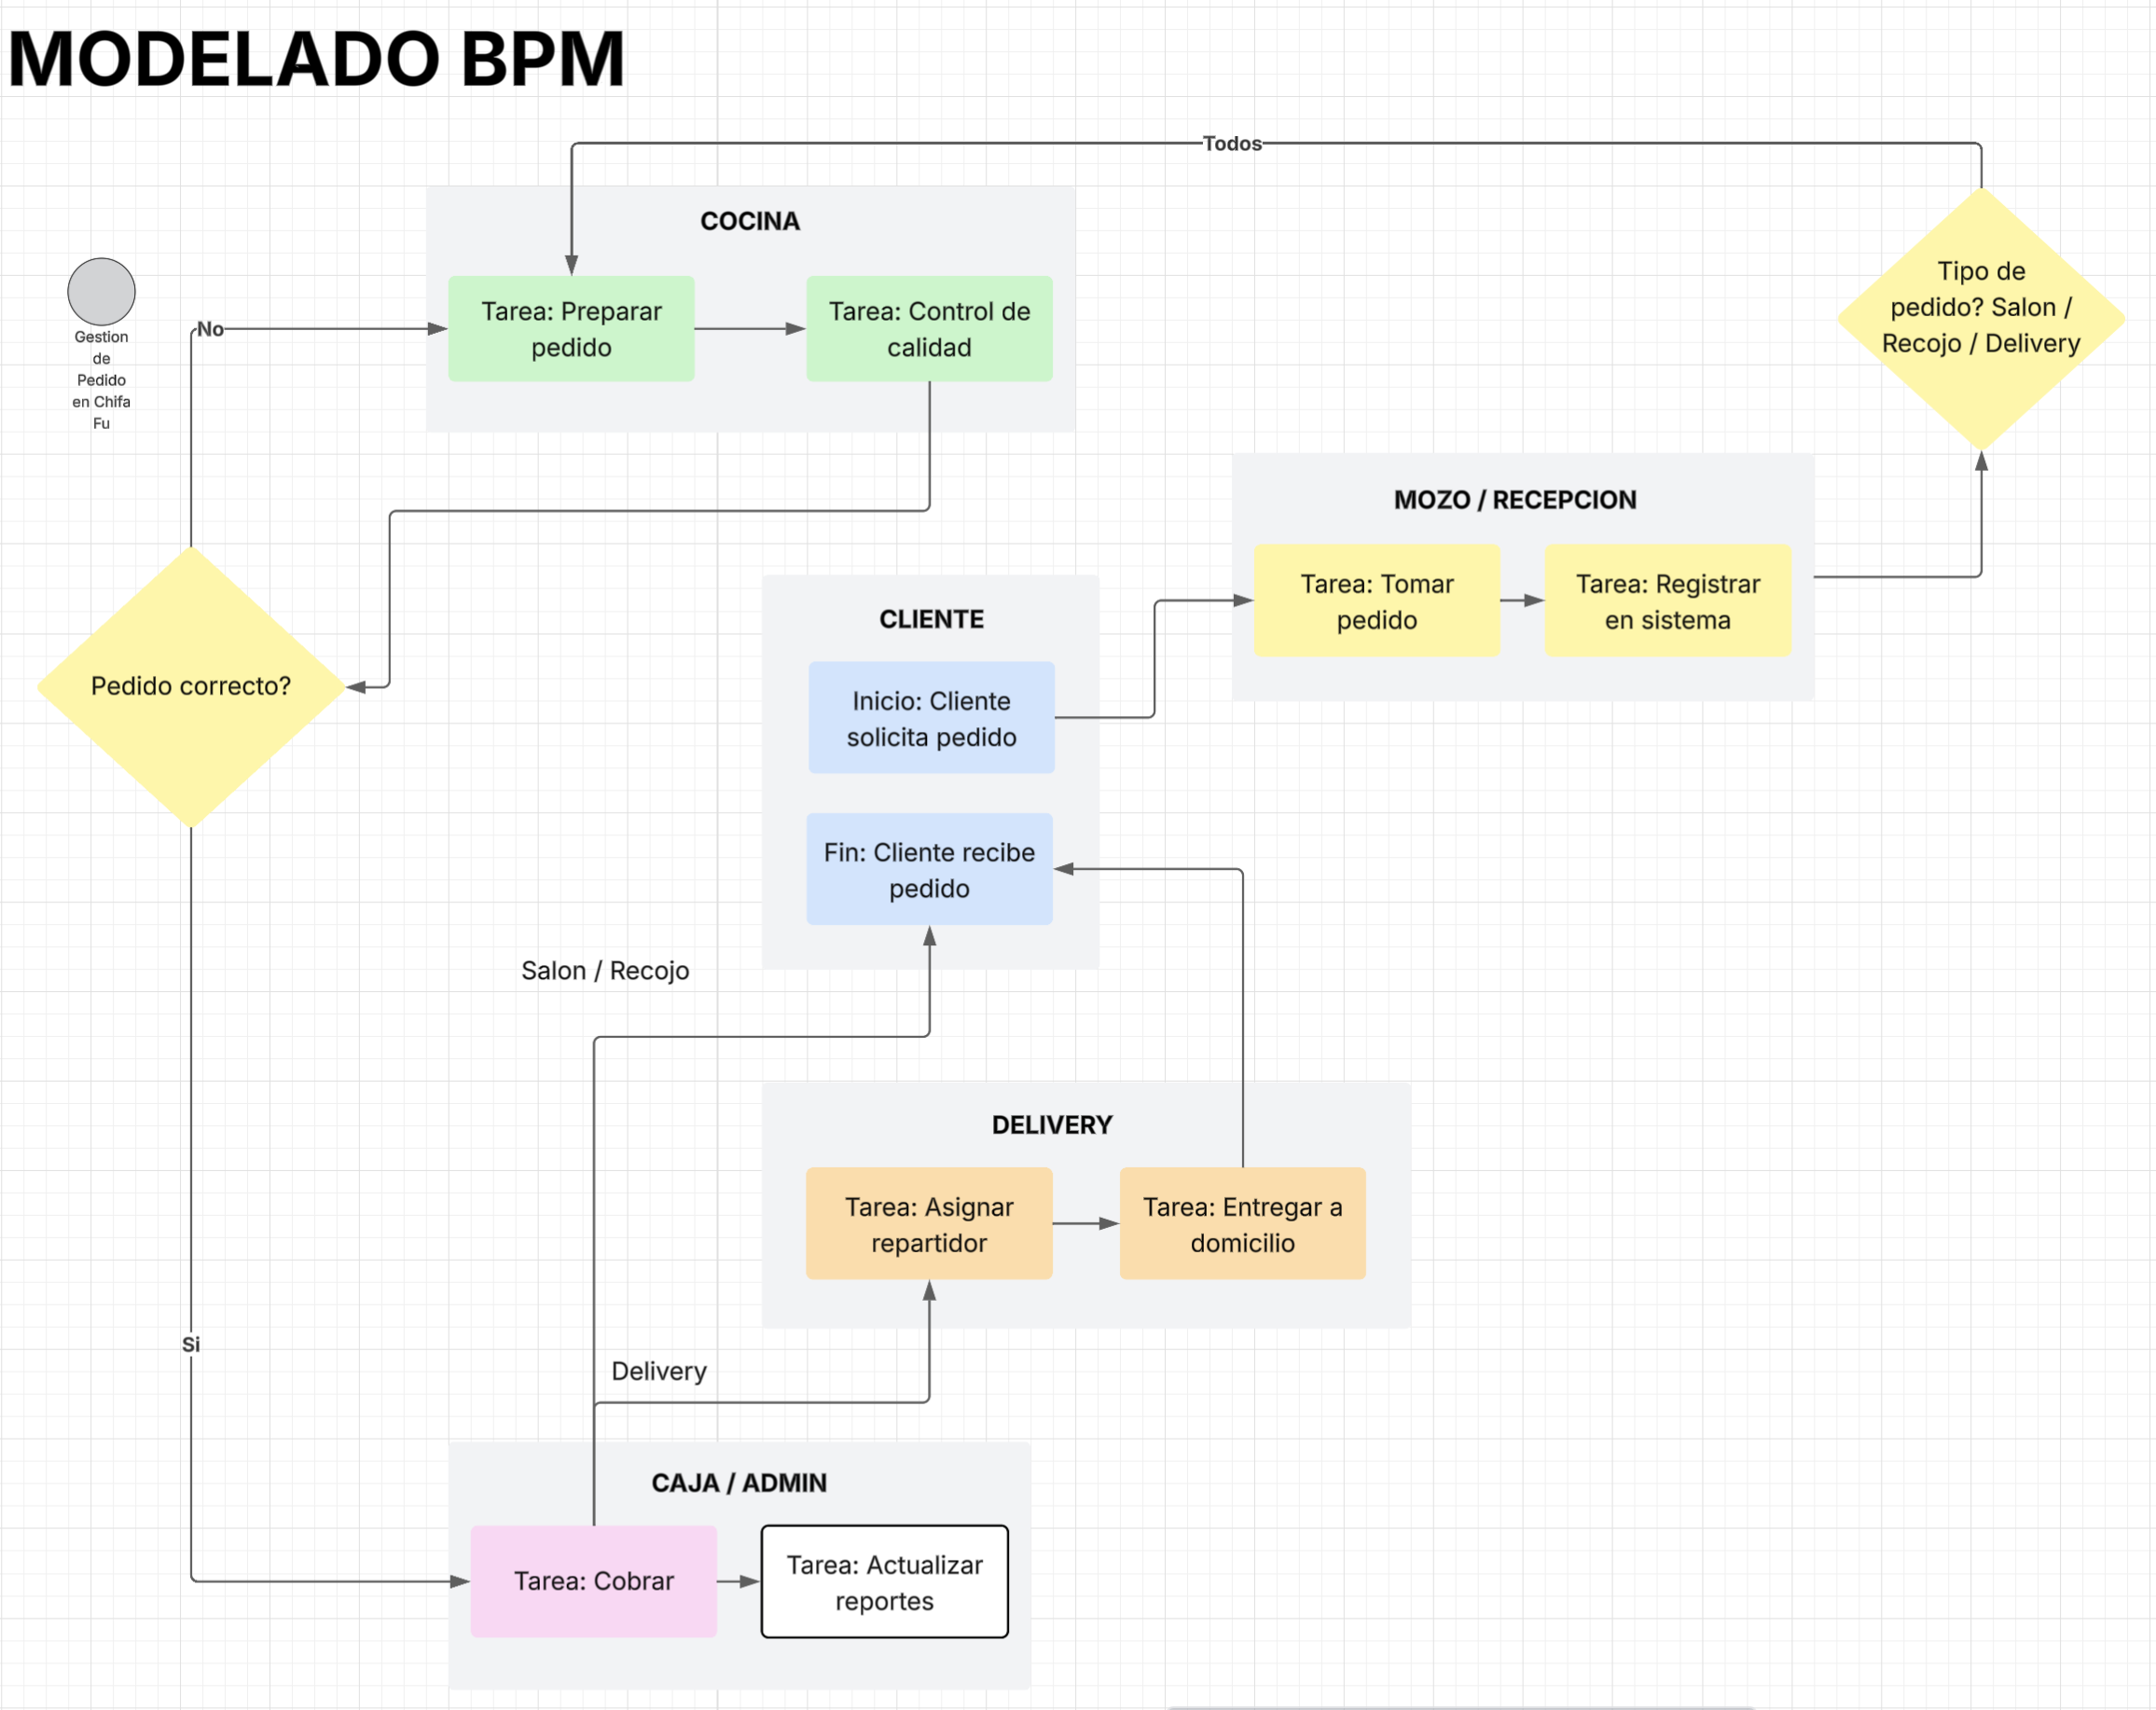
\includegraphics[width=14cm]{Gantt, WBS, Project Charter, BPM/MODELADO BPM.png}
            \caption{Modelado BPM}
            \label{fig:Modelado-BPM}
        \end{figure}
    \end{itemize}

    \section{Diagrama de procesos}
    \begin{itemize}
        \begin{figure}[H]
            \centering
            \vspace*{1cm}
            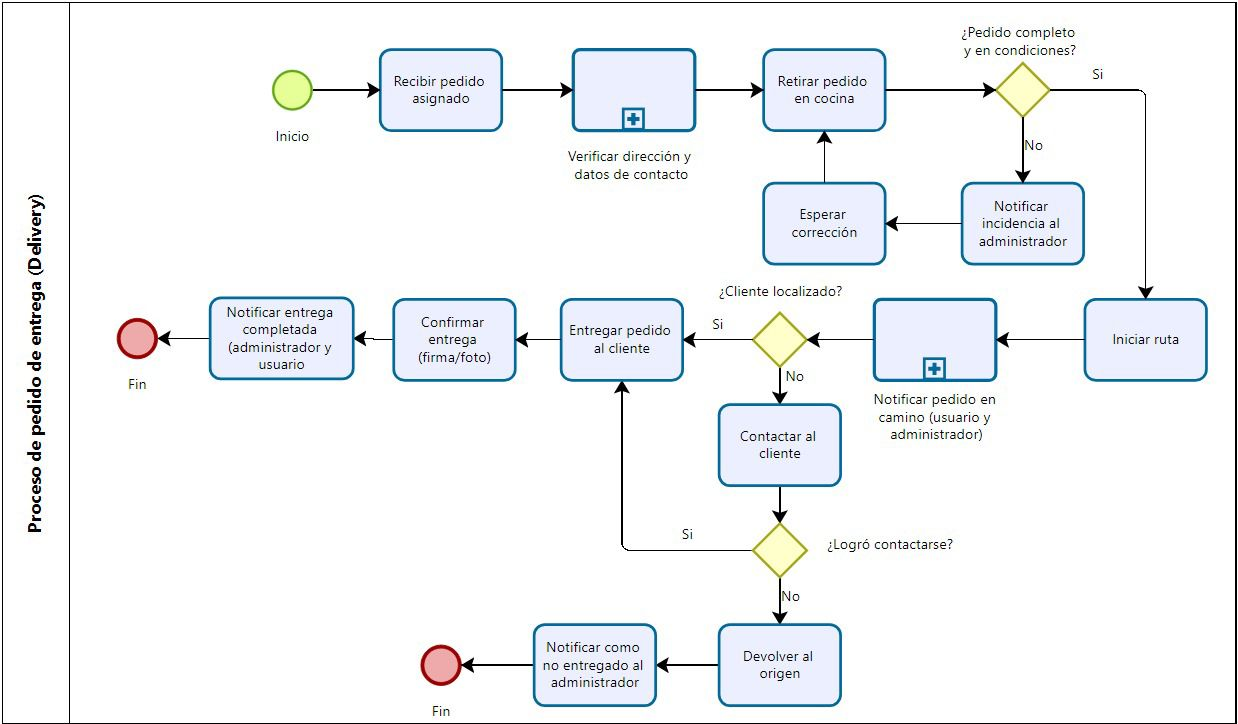
\includegraphics[width=14cm]{Diagrama de Procesos/Proceso de pedido de entrega.jpg}
            \caption{Proceso de pedido de entrega}
            \label{fig:proceso-pedido-de-entrega}
        \end{figure}

        \begin{figure}[H]
            \centering
            \vspace*{1cm}
            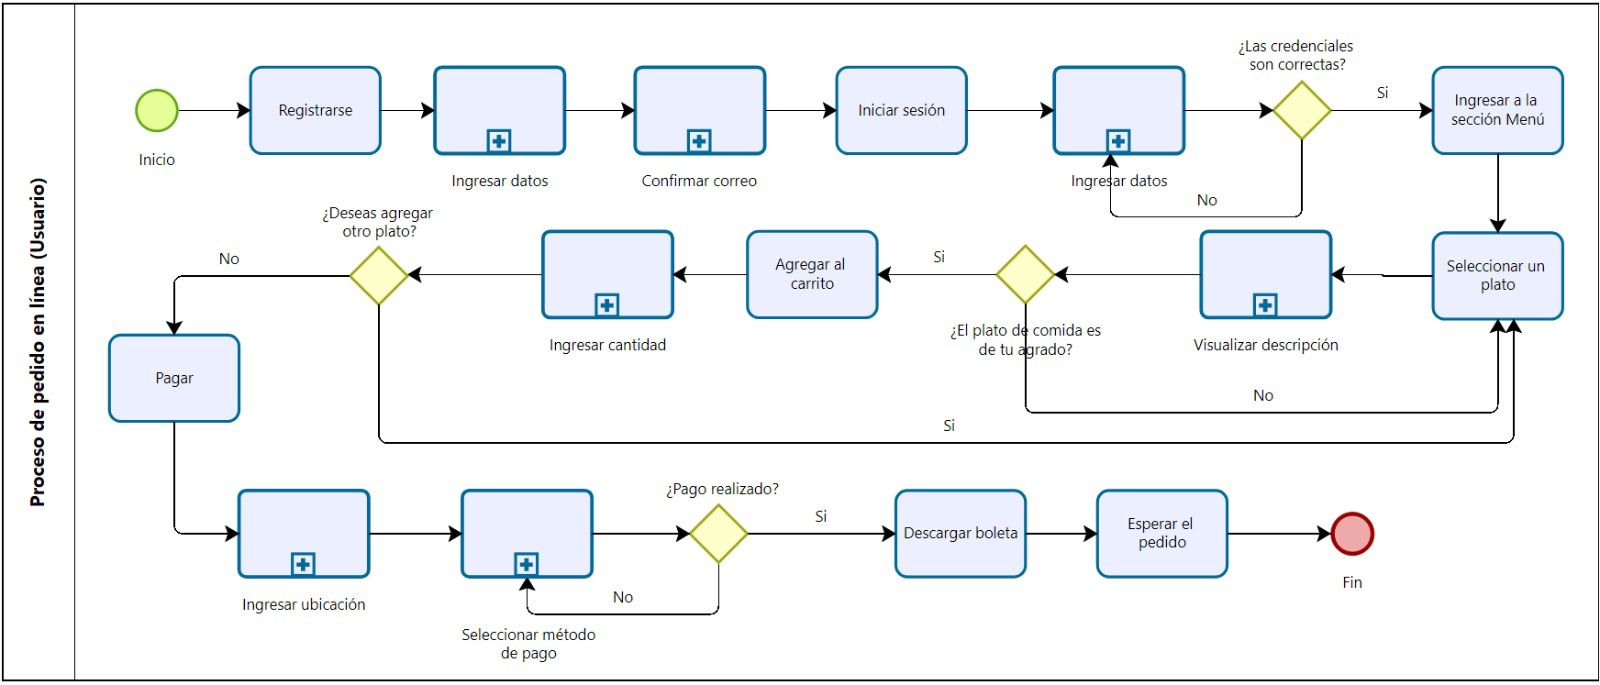
\includegraphics[width=14cm]{Diagrama de Procesos/Proceso de pedido en linea.jpg}
            \caption{Proceso de pedido en linea}
            \label{fig:proceso-pedido-en-linea}
        \end{figure}
    \end{itemize}

    \begin{center}
        \textbf{Este informe fue creado utilizando \LaTeX, un sistema de composición tipográfica muy utilizado en la escritura académica y científica.}
    \end{center}

\end{doublespace}
\end{document}
